\documentclass{article}

% Language and Encoding
\usepackage[english]{babel}
\usepackage[utf8]{inputenc}
\usepackage[T1]{fontenc}

% Fonts
\usepackage{ebgaramond}
\usepackage{lmodern}
\renewcommand*\familydefault{\sfdefault}

% Page Layout
\usepackage[margin=0.7in]{geometry}
\usepackage{microtype}
\usepackage[parfill]{parskip}

% Graphics and Colors
\usepackage{graphicx}
\usepackage{subfig}
\usepackage{xcolor}

% Hyperlinks
\usepackage[hidelinks]{hyperref}

% Headers and Footers
\usepackage{fancyhdr}
\pagestyle{fancy}

% Mathematics
\usepackage{amsmath}

% Code Listings
\usepackage{listings}

% Lists and Enumerations
\usepackage{enumitem}
\setlist[itemize]{leftmargin=*} 

% Miscellaneous
\usepackage{spverbatim}
\usepackage{cprotect}
\usepackage{lipsum}

\usepackage{ebgaramond}

% Title Sections with Enhanced Formatting
\usepackage{titlesec}
\titleformat{\subsubsubsection}
{\normalfont\normalsize\bfseries}{\thesubsubsubsection}{1em}{}
\titlespacing*{\subsubsubsection}
{0pt}{5.5ex plus 1ex minus .2ex}{4.3ex plus .2ex}

% Sectioning support for 'subsubsubsection' using titlesec
\usepackage{titlesec}

\titleformat{\subsubsubsection}
  {\normalfont\normalsize\bfseries\itshape}
  {\thesubsubsubsection}
  {1em}
  {}
\titlespacing*{\subsubsubsection}
{0pt}{3.5ex plus 1ex minus .2ex}{2.3ex plus .2ex}

\makeatletter
\newcounter{subsubsubsection}[subsubsection]
\renewcommand\thesubsubsubsection{\thesubsubsection.\@arabic\c@subsubsubsection}
\newcommand*\l@subsubsubsection{\@dottedtocline{4}{7.0em}{4.1em}}
\makeatother
\setcounter{secnumdepth}{4}
\setcounter{tocdepth}{4}

% Custom Command for Questionnaire Style
\newcommand{\question}[1]{\section*{#1}}
\newcommand{\answer}[1]{\noindent\textit{#1}\par}

% Enhanced Coq codeblocks using lstlisting
\usepackage{listings}
\usepackage{xcolor} % Required for custom colors

% Define a soft color palette
\definecolor{codegreen}{rgb}{0,0.6,0}
\definecolor{codegray}{rgb}{0.5,0.5,0.5}
\definecolor{codepurple}{rgb}{0.58,0,0.82}
\definecolor{backcolor}{rgb}{0.95,0.95,0.92}
\definecolor{codeblue}{rgb}{0,0.1,0.9}

\lstdefinelanguage{Coq}{
  keywords={Definition, Inductive, Fixpoint, match, with, end, as, return, forall, exists, if, then, else, fun, Lemma, Proof, Qed, intro, intros, Theorem},
  morecomment=[s]{(*}{*)},
  morekeywords=[2]{Definition, Inductive, Fixpoint, Lemma, Proof, Qed, Theorem}, % Separate style for special keywords
}

\lstset{
  language=Coq,
  basicstyle=\footnotesize\ttfamily,
  backgroundcolor=\color{backcolor}, 
  commentstyle=\color{codegray}\ttfamily\itshape,
  keywordstyle=\color{codeblue},
  keywordstyle=[2]\color{codepurple}\bfseries, % Apply styling specific to special keywords
  numberstyle=\tiny\color{codegray},
  rulecolor=\color{black},
  breaklines=true,
  frame=tb,
  rulesepcolor=\color{codegreen},
  captionpos=b,
  numbers=none, 
  numbersep=8pt,
  showstringspaces=false,
  stringstyle=\color{codegreen},
  tabsize=2,
  extendedchars=true
}

\usepackage{bookmark} % More modern than hyperref's bookmarks
\bookmarksetup{
  open,
  numbered,
  addtohook={%
    \ifnum\bookmarkget{level}=3 %
      \bookmarksetup{level=4}%
    \fi
  },
}

\title{
    \fontfamily{ebgaramond}\selectfont Midterm Report: Into the Depths of Proofs and Lists \\
    \vspace{1cm}
    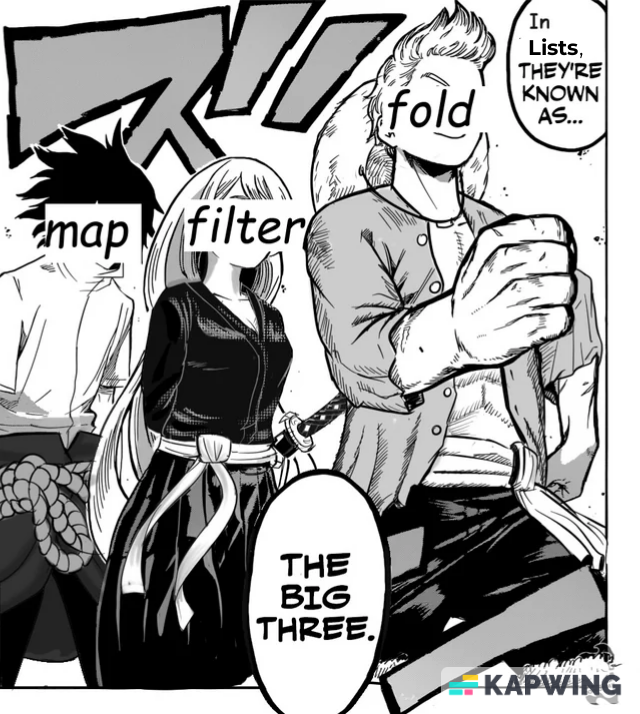
\includegraphics[width=0.8\linewidth]{Untitled_Project_V1.png}
}
\author{YSC3236: Functional Programming and Proving}
\date{%
    \small\emph{"In the world of functional programming, to implement a list is but the first step; to prove its methods is to truly understand its essence."} \\
    - Alan Matthew \\
    \vspace{1cm}
    \today
}

\begin{document}
\maketitle

% Group member details
\newpage
\section*{Group Member Details}
\begin{itemize}
    \item Alan Matthew \\
    Email: alan.matthew@u.yale-nus.edu.sg \\
    Matriculation ID: A0224197B

    \item Jingyi Hou \\
    Email: jingyi.hou@u.yale-nus.edu.sg \\
    Matriculation ID: A0242429E

    \item Sean Lim \\
    Email: sean.lim@u.yale-nus.edu.sg \\
    Matriculation ID: 345678

    \item Zhu Wentao \\
    Email: zhu.wentao@u.yale-nus.edu.sg \\
    Matriculation ID: A0224190N
\end{itemize}
\newpage
\tableofcontents
\newpage

\section{Introduction}

\section{Task 1: A Predicate for Comparing Polymorphic Lists}

\subsection{Question}

In Task 1, we are provided with the function to compare whether two polymorphic lists are equivalent and their fold-unfold lemmas. 

\begin{lstlisting}
Fixpoint eqb_list (V : Type) (eqb_V : V -> V -> bool) (v1s v2s : list V) : bool :=
  match v1s with
  | nil =>
    match v2s with
    | nil =>
      true
    | v2 :: v2s' =>
      false
    end
  | v1 :: v1s' =>
    match v2s with
    | nil =>
      false
    | v2 :: v2s' =>
      eqb_V v1 v2 && eqb_list V eqb_V v1s' v2s'
    end
  end.

Lemma fold_unfold_eqb_list_nil :
  forall (V : Type)
         (eqb_V : V -> V -> bool)
         (v2s : list V),
    eqb_list V eqb_V nil v2s =
    match v2s with
    | nil =>
      true
    | v2 :: v2s' =>
      false
    end.
Proof.
  fold_unfold_tactic eqb_list.
Qed.

Lemma fold_unfold_eqb_list_cons :
  forall (V : Type)
         (eqb_V : V -> V -> bool)
         (v1 : V)
         (v1s' v2s : list V),
    eqb_list V eqb_V (v1 :: v1s') v2s =
    match v2s with
    | nil =>
      false
    | v2 :: v2s' =>
      eqb_V v1 v2 && eqb_list V eqb_V v1s' v2s'
    end.
Proof.
  fold_unfold_tactic eqb_list.
Qed.
\end{lstlisting}

Note that the \texttt{eqb\_list} function is parameterized both by type and by a predicate to compare values of that type. 

We will need to prove the soundness and completeness of the \texttt{eqb\_list} function.

\subsection{Answer}
\subsubsection{Soundness of \texttt{eqb\_list}}

First, we prove the soundness of \texttt{eqb\_list}. Here, the soundness of the \texttt{eqb\_list} function means that if applying the predicate to two values yields \texttt{true}, then these two values must be Leibniz-equal. 

\begin{lstlisting}
Theorem soundness_of_equality_over_lists :
  forall (V : Type)
         (eqb_V : V -> V -> bool),
    (forall v1 v2 : V,
        eqb_V v1 v2 = true -> v1 = v2) ->
    forall v1s v2s : list V,
      eqb_list V eqb_V v1s v2s = true ->
      v1s = v2s.
\end{lstlisting}

First, we need to introduce the parameters of the theorem \texttt{V}, \texttt{eqb\_V} and the hypothesis \texttt{H\_v1\_v2} and \texttt{v1s} into the proof. 

\begin{lstlisting}
1 goal (ID 15)

V : Type
eqb_V : V -> V -> bool
H_v1_v2 : forall v1 v2 : V, eqb_V v1 v2 = true -> v1 = v2
v1s : list V
============================
forall v2s : list V, eqb_list V eqb_V v1s v2s = true -> v1s = v2s
\end{lstlisting}

Next, we use the Light of Inductil and induct on \texttt{v1s}.

\begin{lstlisting}
2 goals (ID 19)

V : Type
eqb_V : V -> V -> bool
H_v1_v2 : forall v1 v2 : V, eqb_V v1 v2 = true -> v1 = v2
============================
forall v2s : list V, eqb_list V eqb_V nil v2s = true -> nil = v2s

goal 2 (ID 23) is:
forall v2s : list V, eqb_list V eqb_V (v1 :: v1s') v2s = true -> v1 :: v1s' = v2s
\end{lstlisting}

We can proceed to the first subgoal. Since we shall be working with \texttt{v2s}, we can introduce the relevant variable and hypothesis and split the list into its head and tail.

\begin{lstlisting}
2 goals (ID 34)

V : Type
eqb_V : V -> V -> bool
H_v1_v2 : forall v1 v2 : V, eqb_V v1 v2 = true -> v1 = v2
H_v1s_v2s : eqb_list V eqb_V nil nil = true
============================
nil = nil

goal 2 (ID 37) is:
nil = v2 :: v2s'
\end{lstlisting}

Focusing on the base case

\begin{lstlisting}
1 goal (ID 34)

V : Type
eqb_V : V -> V -> bool
H_v1_v2 : forall v1 v2 : V, eqb_V v1 v2 = true -> v1 = v2
H_v1s_v2s : eqb_list V eqb_V nil nil = true
============================
nil = nil
\end{lstlisting}

It can be proven using the \texttt{reflexivity} tactic. Proceeding to the next subgoal:

\begin{lstlisting}
1 goal (ID 37)

V : Type
eqb_V : V -> V -> bool
H_v1_v2 : forall v1 v2 : V, eqb_V v1 v2 = true -> v1 = v2
v2 : V
v2s' : list V
H_v1s_v2s : eqb_list V eqb_V nil (v2 :: v2s') = true
============================
nil = v2 :: v2s'
\end{lstlisting}

Which is an instance of the \texttt{fold\_unfold\_eqb\_list\_nil} lemma applied to \texttt{V}, \texttt{eqb\_V}, and \texttt{(v2::v2s')} in \texttt{H\_v1s\_v2s}. 

\begin{lstlisting}
1 goal (ID 41)

V : Type
eqb_V : V -> V -> bool
H_v1_v2 : forall v1 v2 : V, eqb_V v1 v2 = true -> v1 = v2
v2 : V
v2s' : list V
H_v1s_v2s : false = true
============================
nil = v2 :: v2s'
\end{lstlisting}

We can observe in the environment that \texttt{H\_v1s\_v2s : false = true} is clearly absurd. We can prove this by applying the \texttt{discriminate} tactic on \texttt{H\_v1s\_v2s}.

Repeating the same process for the next subgoal reads:

\begin{lstlisting}
1 goal (ID 55)

V : Type
eqb_V : V -> V -> bool
H_v1_v2 : forall v1 v2 : V, eqb_V v1 v2 = true -> v1 = v2
v1 : V
v1s' : list V
IHv1s' : forall v2s : list V, eqb_list V eqb_V v1s' v2s = true -> v1s' = v2s
H_v1s_v2s : eqb_list V eqb_V (v1 :: v1s') nil = true
============================
v1 :: v1s' = nil
\end{lstlisting}

Focusing on the left-hand side of the equation, it is an instance of \texttt{fold\_unfold\_eqb\_list\_cons} applied to \texttt{V}, \texttt{eqb\_V}, \texttt{v1}, \texttt{v1s'}, and \texttt{nil} in \texttt{H\_v1s\_v2s}.

\begin{lstlisting}
1 goal (ID 61)

V : Type
eqb_V : V -> V -> bool
H_v1_v2 : forall v1 v2 : V, eqb_V v1 v2 = true -> v1 = v2
v1 : V
v1s' : list V
IHv1s' : forall v2s : list V, eqb_list V eqb_V v1s' v2s = true -> v1s' = v2s
H_v1s_v2s : false = true
============================
v1 :: v1s' = nil
\end{lstlisting}

In the environment, we can observe that \texttt{H\_v1s\_v2s : false = true} is clearly absurd. We can prove this by applying the \texttt{discriminate} tactic on \texttt{H\_v1s\_v2s}.

\begin{lstlisting}
1 goal (ID 58)

V : Type
eqb_V : V -> V -> bool
H_v1_v2 : forall v1 v2 : V, eqb_V v1 v2 = true -> v1 = v2
v1 : V
v1s' : list V
IHv1s' : forall v2s : list V, eqb_list V eqb_V v1s' v2s = true -> v1s' = v2s
v2 : V
v2s' : list V
H_v1s_v2s : eqb_list V eqb_V (v1 :: v1s') (v2 :: v2s') = true
============================
v1 :: v1s' = v2 :: v2s'
\end{lstlisting}

Similarly, the last goal is an instance of \texttt{fold\_unfold\_eqb\_list\_cons} applied to \texttt{V}, \texttt{eqb\_V}, \texttt{v1}, \texttt{v1s'}, and \texttt{v2::v2s'} in \texttt{H\_v1s\_v2s}.

\begin{lstlisting}
1 goal (ID 67)

V : Type
eqb_V : V -> V -> bool
H_v1_v2 : forall v1 v2 : V, eqb_V v1 v2 = true -> v1 = v2
v1 : V
v1s' : list V
IHv1s' : forall v2s : list V, eqb_list V eqb_V v1s' v2s = true -> v1s' = v2s
v2 : V
v2s' : list V
H_v1s_v2s : eqb_V v1 v2 && eqb_list V eqb_V v1s' v2s' = true
============================
v1 :: v1s' = v2 :: v2s'
\end{lstlisting}

In the environment, \texttt{H\_v1s\_v2s} is a conjunction of two boolean expressions. Using the \texttt{Search} tactic, we can find the \texttt{andb\_prop} lemma to destruct our conjunction into its conjuncts. 

\begin{lstlisting}
1 goal (ID 79)

V : Type
eqb_V : V -> V -> bool
H_v1_v2 : forall v1 v2 : V, eqb_V v1 v2 = true -> v1 = v2
v1 : V
v1s' : list V
IHv1s' : forall v2s : list V, eqb_list V eqb_V v1s' v2s = true -> v1s' = v2s
v2 : V
v2s' : list V
H_v1s_v2s : eqb_V v1 v2 && eqb_list V eqb_V v1s' v2s' = true
v1_equals_v2 : eqb_V v1 v2 = true
v1s'_equals_v2s' : eqb_list V eqb_V v1s' v2s' = true
============================
v1 :: v1s' = v2 :: v2s'
\end{lstlisting}

We can rewrite the subgoal using our conjuncts to help complete the proof. In the first rewrite, \texttt{H\_v1\_v2} is applied to \texttt{v1}, \texttt{v2}, and \texttt{v1\_equals\_v2} to yield \texttt{v1 = v2}. In the second rewrite, \texttt{IHv1s'} is applied to \texttt{v1s'\_equals\_v2s'} to yield \texttt{v1s' = v2s'}. With that, the proof can be completed using the \texttt{reflexivity} tactic.

Here is the full proof for reference:

\begin{lstlisting}
Theorem soundness_of_equality_over_lists :
  forall (V : Type)
         (eqb_V : V -> V -> bool),
    (forall v1 v2 : V,
        eqb_V v1 v2 = true -> v1 = v2) ->
    forall v1s v2s : list V,
      eqb_list V eqb_V v1s v2s = true ->
      v1s = v2s.
Proof.
  intros V eqb_V H_v1_v2 v1s.
  induction v1s as [ | v1 v1s' IHv1s'].
  + intros v2s H_v1s_v2s.
    case v2s as [ | v2 v2s'].
    ++
      reflexivity.
    ++ rewrite -> (fold_unfold_eqb_list_nil V eqb_V (v2 :: v2s')) in H_v1s_v2s.
       discriminate H_v1s_v2s.
  + intros v2s H_v1s_v2s.
    case v2s as [ | v2 v2s'].
    ++ rewrite -> (fold_unfold_eqb_list_cons V eqb_V v1 v1s' nil) in H_v1s_v2s.
       discriminate H_v1s_v2s.
    ++ rewrite -> (fold_unfold_eqb_list_cons V eqb_V v1 v1s' (v2 :: v2s')) in H_v1s_v2s.
       Search (_ && _ = true).
       destruct (andb_prop (eqb_V v1 v2) (eqb_list V eqb_V v1s' v2s') (H_v1s_v2s)) as [v1_equals_v2 v1s'_equals_v2s'].
       rewrite -> (H_v1_v2 v1 v2 v1_equals_v2).
       rewrite -> (IHv1s' v2s' v1s'_equals_v2s').
       reflexivity.
Qed.
\end{lstlisting}

\subsubsection{Completeness of \texttt{eqb\_list}}
Secondly, we prove the completeness of \texttt{eqb\_list}. Here, the completeness of the \texttt{eqb\_list} function means that if two values are Leibniz-equal, then applying the predicate to these two values yields \texttt{true}.

\begin{lstlisting}
Theorem completeness_of_equality_over_lists :
  forall (V : Type)
         (eqb_V : V -> V -> bool),
    (forall v1 v2 : V,
        v1 = v2 -> eqb_V v1 v2 = true) ->
    forall v1s v2s : list V,
      v1s = v2s ->
      eqb_list V eqb_V v1s v2s = true.
\end{lstlisting}

Similar to the proof for soundness, we introduce the parameters of the theorem \texttt{V}, \texttt{eqb\_V} and the hypothesis \texttt{H\_v1\_v2} and \texttt{v1s} into the proof and then proceed with induction in the form Light of Inductil.

\begin{lstlisting}
2 goals (ID 24)

V : Type
eqb_V : V -> V -> bool
H_v1_v2 : forall v1 v2 : V, v1 = v2 -> eqb_V v1 v2 = true
============================
forall v2s : list V, nil = v2s -> eqb_list V eqb_V nil v2s = true

goal 2 (ID 28) is:
forall v2s : list V, v1 :: v1s' = v2s -> eqb_list V eqb_V (v1 :: v1s') v2s = true
\end{lstlisting}

The first three subgoals are similar to the steps taken in the soundness proof or solvable in one step. We shall omit the proofs for these subgoals here for brevity.

Proceeding to the last subgoal:

\begin{lstlisting}
1 goal (ID 62)

V : Type
eqb_V : V -> V -> bool
H_v1_v2 : forall v1 v2 : V, v1 = v2 -> eqb_V v1 v2 = true
v1 : V
v1s' : list V
IHv1s' : forall v2s : list V, v1s' = v2s -> eqb_list V eqb_V v1s' v2s = true
v2 : V
v2s' : list V
H_v1s_v2s : v1 :: v1s' = v2 :: v2s'
============================
eqb_list V eqb_V (v1 :: v1s') (v2 :: v2s') = true  
\end{lstlisting}

Firstly, we can simplify the goal and rewrite (v2::v2s') to (v1::v1s') using \texttt{H\_v1s\_v2s}.

\begin{lstlisting}
1 goal (ID 65)

V : Type
eqb_V : V -> V -> bool
H_v1_v2 : forall v1 v2 : V, v1 = v2 -> eqb_V v1 v2 = true
v1 : V
v1s' : list V
IHv1s' : forall v2s : list V, v1s' = v2s -> eqb_list V eqb_V v1s' v2s = true
v2 : V
v2s' : list V
H_v1s_v2s : v1 :: v1s' = v2 :: v2s'
============================
eqb_list V eqb_V (v1 :: v1s') (v1 :: v1s') = true
\end{lstlisting}

The goal becomes an instance of \texttt{fold\_unfold\_eqb\_list\_cons} applied to \texttt{V}, \texttt{eqb\_V}, \texttt{v1}, \texttt{v1s'}, and \texttt{v1::v1s'}.

Since the goal is a conjunction, using the \texttt{Search} tactic helps us find the \texttt{andb\_true\_iff} lemma to destruct our conjunction into its conjuncts.

\begin{lstlisting}
1 goal (ID 80)

V : Type
eqb_V : V -> V -> bool
H_v1_v2 : forall v1 v2 : V, v1 = v2 -> eqb_V v1 v2 = true
v1 : V
v1s' : list V
IHv1s' : forall v2s : list V, v1s' = v2s -> eqb_list V eqb_V v1s' v2s = true
v2 : V
v2s' : list V
H_v1s_v2s : v1 :: v1s' = v2 :: v2s'
H_tmp : eqb_V v1 v1 = true /\ eqb_list V eqb_V v1s' v1s' = true ->
        eqb_V v1 v1 && eqb_list V eqb_V v1s' v1s' = true
============================
eqb_V v1 v1 && eqb_list V eqb_V v1s' v1s' = true
\end{lstlisting}

Since the implication of \texttt{H\_tmp} matches the goal, we can use the \texttt{apply} tactic to apply \texttt{H\_tmp} to the goal and split the conjunction.

The first subgoal of this is: 

\begin{lstlisting}
1 goal (ID 83)

V : Type
eqb_V : V -> V -> bool
H_v1_v2 : forall v1 v2 : V, v1 = v2 -> eqb_V v1 v2 = true
v1 : V
v1s' : list V
IHv1s' : forall v2s : list V, v1s' = v2s -> eqb_list V eqb_V v1s' v2s = true
v2 : V
v2s' : list V
H_v1s_v2s : v1 :: v1s' = v2 :: v2s'
H_tmp : eqb_V v1 v1 = true /\ eqb_list V eqb_V v1s' v1s' = true ->
        eqb_V v1 v1 && eqb_list V eqb_V v1s' v1s' = true
============================
eqb_V v1 v1 = true
\end{lstlisting}

Since the implication of \texttt{H\_v1\_v2} matches the goal, we can use the \texttt{apply} tactic to apply \texttt{H\_v1\_v2} to the goal and complete the subgoal using the \texttt{reflexivity} tactic.

\begin{lstlisting}
1 goal (ID 84)

V : Type
eqb_V : V -> V -> bool
H_v1_v2 : forall v1 v2 : V, v1 = v2 -> eqb_V v1 v2 = true
v1 : V
v1s' : list V
IHv1s' : forall v2s : list V, v1s' = v2s -> eqb_list V eqb_V v1s' v2s = true
v2 : V
v2s' : list V
H_v1s_v2s : v1 :: v1s' = v2 :: v2s'
H_tmp : eqb_V v1 v1 = true /\ eqb_list V eqb_V v1s' v1s' = true ->
        eqb_V v1 v1 && eqb_list V eqb_V v1s' v1s' = true
============================
eqb_list V eqb_V v1s' v1s' = true
\end{lstlisting}

Similarly, the last subgoal matches the implication of the induction hypothesis \texttt{IHv1s'} and we can use the \texttt{apply} tactic to apply \texttt{IHv1s'} to the goal and complete the subgoal using the \texttt{reflexivity} tactic.

Here is the full proof for reference:

\begin{lstlisting}
Theorem completeness_of_equality_over_lists :
  forall (V : Type)
         (eqb_V : V -> V -> bool),
    (forall v1 v2 : V,
        v1 = v2 -> eqb_V v1 v2 = true) ->
    forall v1s v2s : list V,
      v1s = v2s ->
      eqb_list V eqb_V v1s v2s = true.
Proof.
  intros V eqb_V H_v1_v2 v1s.
  induction v1s as [ | v1 v1s' IHv1s'].
  + intros v2s H_v1s_v2s.
     case v2s as [ | v2 v2s'].
     ++ rewrite -> (fold_unfold_eqb_list_nil V eqb_V nil).
         reflexivity.
     ++ discriminate H_v1s_v2s.
  + intros v2s H_v1s_v2s.
    case v2s as [ | v2 v2s'].
    ++ discriminate H_v1s_v2s.
    ++ rewrite <- H_v1s_v2s.
       rewrite -> (fold_unfold_eqb_list_cons V eqb_V v1 v1s' (v1 :: v1s')).
       Search (_ && _ = true).
       destruct (andb_true_iff (eqb_V v1 v1) (eqb_list V eqb_V v1s' v1s')) as [_ H_tmp].
       apply H_tmp.
       split.
       +++
         apply (H_v1_v2 v1 v1).
         reflexivity.
       +++
         apply (IHv1s' v1s').
         reflexivity.
Qed.    
\end{lstlisting}  

\subsection{Conclusion}

In Task 1, the proof of soundness and completeness of the \texttt{eqb\_list} function was relatively routine and straightforward, following the same patters we have encountered in the weekly exercises so far. However, the value in Task 1 is in familiarizing ourselves with lists and the \texttt{apply} and \texttt{discriminate} tactics for the midterm project and beyond.

\newpage

\section{Task 2: The Length of a Polymporphic List}

\subsection{Question}

In Task 2, we are asked to implement a recursive function to compute the length of a polymorphic list using an accumulator. Furthermore, we must prove that the implementation indeed satisfies the specification of the length function.

We are provided with some examples for the implementation of list length function without using an accumulator, but I will omit them here for brevity except for the specification and unit test. 

\begin{lstlisting}
(* A study of the polymorphic length function: *)

Definition specification_of_list_length (length : forall V : Type, list V -> nat) :=
  (forall V : Type,
      length V nil = 0)
  /\
  (forall (V : Type)
          (v : V)
          (vs' : list V),
     length V (v :: vs') = S (length V vs')).

(* Unit-test function: *)

Definition test_list_length (candidate : forall V : Type, list V -> nat) :=
  (candidate nat nil =? 0) &&
    (candidate bool nil =? 0) &&
    (candidate nat (1 :: nil) =? 1) &&
    (candidate bool (true :: nil) =? 1) &&
    (candidate nat (2 :: 1 :: nil) =? 2) &&
    (candidate bool (false :: true :: nil) =? 2) &&
    (candidate nat (3 :: 2 :: 1 :: nil) =? 3) &&
    (candidate bool (false :: false :: true :: nil) =? 3) &&
    (candidate nat (5 :: 4 :: 3 :: 2 :: 1 :: nil) =? 5) &&
    (candidate bool (true :: true :: false :: false :: true :: nil) =? 5).
\end{lstlisting}

\subsection{Answer}

The first step to implement the recursive function to compute the length of a polymorphic list using an accumulator. The implementation is quite straightforward where we use the accumulator \texttt{a} to keep track of the length of the list. With our recursive implementation, we can wrap it in a function that takes in a list and returns the length of the list.

\begin{lstlisting}
(* Implement the length function using an accumulator. *)

Fixpoint list_length_acc (V : Type) (ls : list V) (a : nat) : nat :=
  match ls with
  | nil =>
      a
  | v :: vs' =>
      list_length_acc V vs' (S a)
  end.


Definition list_length_alt (V : Type) (vs : list V) : nat :=
  list_length_acc V vs 0.

Compute (test_list_length list_length_alt).
(* 
= true
: bool
*)
\end{lstlisting}

Since we implemented a recursive function, it is best practice to implement its respective fold-unfold lemmas for the base case and the inductive case.

\begin{lstlisting}
Lemma fold_unfold_list_length_acc_nil :
  forall (V : Type)
         (acc : nat),
    list_length_acc V nil acc =
      acc.
Proof.
  fold_unfold_tactic list_length_acc.
Qed.

Lemma fold_unfold_list_length_acc_cons :
  forall (V : Type)
         (v : V)
         (vs' : list V)
         (acc : nat),
    list_length_acc V (v :: vs') acc =
      list_length_acc V vs' (S acc).
Proof.
  fold_unfold_tactic list_length_acc.
Qed.
\end{lstlisting}

Next, we prove that the implementation of the length function indeed satisfies the specification of the length function.

\begin{lstlisting}
Theorem list_length_alt_satisfies_the_specification_of_list_length :
  specification_of_list_length list_length_alt.
\end{lstlisting}

Similar to the exercises from our previous weeks, we must first unfold the specifications in the theorem.

\begin{lstlisting}
1 goal (ID 71)

============================
(forall V : Type, list_length_acc V nil 0 = 0) /\
(forall (V : Type) (v : V) (vs' : list V),
  list_length_acc V (v :: vs') 0 = S (list_length_acc V vs' 0))
\end{lstlisting}

The goal shows a conjunction. We can use the \texttt{split} tactic to split the goal into two subgoals. Let us observe the first.

\begin{lstlisting}
1 goal (ID 73)

============================
forall V : Type, list_length_acc V nil 0 = 0
\end{lstlisting}

The goal is an instance of the \texttt{fold\_unfold\_list\_length\_acc\_nil} lemma applied to \texttt{V} and \texttt{0}. We can prove this by applying the \texttt{reflexivity} tactic.

\begin{lstlisting}
1 goal (ID 80)

V : Type
v : V
vs' : list V
============================
list_length_acc V (v :: vs') 0 = S (list_length_acc V vs' 0)
\end{lstlisting}

The goal currently shows an instance of the fold-unfold lemma for the list length using an accumulator function. We can rewrite the goal using \texttt{fold\_unfold\_list\_length\_acc\_cons} lemma applied to \texttt{V}, \texttt{v}, \texttt{vs'}, and \texttt{0}.

\begin{lstlisting}
1 goal (ID 81)

V : Type
v : V
vs' : list V
============================
list_length_acc V vs' 1 = S (list_length_acc V vs' 0)
\end{lstlisting}

The goal reads that the length of the list \texttt{vs'} with an accumulator of \texttt{1} is equal to the succession of the length of the list \texttt{vs'} with an accumulator of \texttt{0}. We can postulate this lemma and see if it helps us complete the proof.

\begin{lstlisting}
Lemma list_length_S_acc_equals_S_list_length : 
  forall (V: Type)
         (v : V)
         (vs' : list V)
         (acc : nat),
    list_length_acc V vs' (S acc) = S (list_length_acc V vs' acc).
Proof.
Admitted.
\end{lstlisting}

Proceeding with our original proof:

\begin{lstlisting}
1 goal (ID 82)

V : Type
v : V
vs' : list V
============================
S (list_length_acc V vs' 0) = S (list_length_acc V vs' 0)
\end{lstlisting}

The lemma does indeed help and we can complete our proof using the \texttt{reflexivity} tactic. Let us return to the proof for the lemma we postulated.

We can first introduce the relevant variables \texttt{V}, \texttt{v}, and \texttt{vs'} into the proof.

\begin{lstlisting}
1 goal (ID 72)

V : Type
v : V
vs' : list V
============================
forall a : nat, list_length_acc V vs' (S a) = S (list_length_acc V vs' a)
\end{lstlisting}

However, since \texttt{v} is not used in the goal, we can remove it using the \texttt{revert} tactic. Furthermore, we can proceed with our proof using induction in the form Light of Inductil.

Focusing on our first subgoal:

\begin{lstlisting}
1 goal (ID 84)

V : Type
v : V
a : nat
============================
list_length_acc V nil (S a) = S (list_length_acc V nil a)
\end{lstlisting}

The left-hand side and right-hand side of the equation are both instances of the \texttt{fold\_unfold\_list\_length\_acc\_nil} lemma applied to \texttt{V} and \texttt{(S a)} and \texttt{a} respectively. This is routine and we can complete the proof for the subgoal using the \texttt{reflexivity} tactic.

The next subgoal reads:

\begin{lstlisting}
1 goal (ID 89)

V : Type
v' : V
vs'' : list V
IHvs'' : V -> forall a : nat, list_length_acc V vs'' (S a) = S (list_length_acc V vs'' a)
v : V
a : nat
============================
list_length_acc V (v' :: vs'') (S a) = S (list_length_acc V (v' :: vs'') a)
\end{lstlisting}

Similar to the previous case, but with an extra step, the left-hand side and right-hand side of the equation are both instances of the \texttt{fold\_unfold\_list\_length\_acc\_cons} lemma applied to \texttt{V}, \texttt{v'}, \texttt{vs''}, and \texttt{(S a)} and \texttt{a} respectively.

\begin{lstlisting}
1 goal (ID 91)

V : Type
v' : V
vs'' : list V
IHvs'' : V -> forall a : nat, list_length_acc V vs'' (S a) = S (list_length_acc V vs'' a)
v : V
a : nat
============================
list_length_acc V vs'' (S (S a)) = S (list_length_acc V vs'' (S a))
\end{lstlisting}

The goal seemingly becomes an instance of the inductive hypothesis \texttt{IHvs''} applied to \texttt{v} and \texttt{(S a)}. We can confirm this using the \texttt{Check} tactic.

\begin{lstlisting}
IHvs'' v (S a)
  : list_length_acc V vs'' (S (S a)) = S (list_length_acc V vs'' (S a))
\end{lstlisting}

We are correct and we can complete our proof using the \texttt{exact} tactic.

Here is the full proof for reference:

\begin{lstlisting}
Lemma list_length_S_acc_equals_S_list_length : 
  forall (V: Type)
         (v : V)
         (vs' : list V)
         (a : nat),
    list_length_acc V vs' (S a) = S (list_length_acc V vs' a).
Proof.
  intros V v vs'.
  revert v.
  induction vs' as [ | v' vs'' IHvs''].
  + intros v a.
    rewrite -> (fold_unfold_list_length_acc_nil V (S a)).
    rewrite -> (fold_unfold_list_length_acc_nil V a).
    reflexivity.
  + intros v a.
    rewrite -> (fold_unfold_list_length_acc_cons V v' vs'' (S a)).
    rewrite -> (fold_unfold_list_length_acc_cons V v' vs'' a).
    Check (IHvs'' v (S a)).
    exact (IHvs'' v (S a)).
Qed.

\end{lstlisting}

\subsection{Conclusion}

Similar to Task 1, the solution for Task 2 are similar to the exercises we completed in the previous weeks. However Task 2 is slightly more difficult than Task 1 as we needed to find an eureka lemma to help us complete the proof. Nonetheless, it was a good exercises to familiarize ourselves with formulating eureka lemmas and working with lists in Gallina.

\newpage

\section{Task 3: Copying a Polymorphic List}

In Task 3, we are asked to implement a recursive function to copy a polymorphic list. Furthermore, we need to prove that the implementation satisfies the specification, is idempotent and preserves the length of the list. Additionally, we also come up with a strikingly simple implementation of the copy function and prove its corresponding properties.

We are provided with the specification of \texttt{list\_copy} and a unit-test function.

\begin{lstlisting}
Definition specification_of_list_copy (copy : forall V : Type, list V -> list V) :=
  (forall V : Type,
      copy V nil = nil)
  /\
    (forall (V : Type)
            (v : V)
            (vs' : list V),
        copy V (v :: vs') = v :: (copy V vs')).

Definition test_list_copy (candidate : forall V : Type, list V -> list V) :=
  (eqb_list nat Nat.eqb (candidate nat nil) nil) &&
    (eqb_list bool Bool.eqb (candidate bool nil) nil) &&
    (eqb_list nat Nat.eqb (candidate nat (1 :: nil)) (1 :: nil)) &&
    (eqb_list bool Bool.eqb (candidate bool (true :: nil)) (true :: nil)) &&
    (eqb_list nat Nat.eqb (candidate nat (2 :: 1 :: nil)) (2 :: 1 :: nil)) &&
    (eqb_list bool Bool.eqb (candidate bool (false :: true :: nil)) (false :: true :: nil)).
\end{lstlisting}

\subsection{Tasks 3a - 3c}

\subsubsection{Question}
We are asked to expand the unit-test function for copy with a few more tests, implement the copy function recursively and state its fold-unfold lemmas.

\subsubsection{Answer}

We begin with adding a few more unit tests.

\begin{lstlisting}
Definition test_list_copy_expanded (candidate : forall V : Type, list V -> list V) :=
  (eqb_list nat Nat.eqb (candidate nat nil) nil) &&
  (eqb_list bool Bool.eqb (candidate bool nil) nil) &&
  (eqb_list nat Nat.eqb (candidate nat (1 :: nil)) (1 :: nil)) &&
  (eqb_list bool Bool.eqb (candidate bool (true :: nil)) (true :: nil)) &&
  (eqb_list nat Nat.eqb (candidate nat (2 :: 1 :: nil)) (2 :: 1 :: nil)) &&
  (eqb_list bool Bool.eqb (candidate bool (false :: true :: nil)) (false :: true :: nil)) &&
  (eqb_list nat Nat.eqb (candidate nat (4 :: 3 :: 2 :: 1 :: nil)) (4 :: 3 :: 2 :: 1 :: nil)) &&
  (eqb_list bool Bool.eqb (candidate bool (true :: false :: false :: true :: nil)) (true :: false :: false :: true :: nil)).
\end{lstlisting}

Then, we implement the function recursively with the nil case as the base case and the cons case as the recursive step by appending the head of the list to the copy of the tail of the list.

\begin{lstlisting}
Fixpoint list_copy (V : Type) (vs : list V) : list V :=
  match vs with
  | nil =>
      nil
  | v :: vs' =>
      v :: list_copy V vs'
  end.

Compute (test_list_copy_expanded list_copy).
\end{lstlisting}

We check that our implementation passes the unit tests, which it does.

Naturally, the fold-unfold lemmas are then stated for the nil case and cons case.

\begin{lstlisting}
Lemma fold_unfold_list_copy_nil :
  forall V : Type,
    list_copy V nil =
      nil.
Proof.
  fold_unfold_tactic list_copy.
Qed.

Lemma fold_unfold_list_copy_cons :
  forall (V : Type)
         (v : V)
         (vs' : list V),
    list_copy V (v :: vs') =
      v :: list_copy V vs'.
Proof.
  fold_unfold_tactic list_copy.
Qed.
\end{lstlisting}

\subsubsection{Conclusion}
In these exercises we wrote unit tests and implemented the copy function for lists recursively, validated it, and stated its fold-unfold lemmas, which are very fundamental steps when asked to implement a function that we should always keep in mind.

\subsection{Task 3d}
\subsubsection{Question}
We are asked the prove that our implementation satisfies the specification of \texttt{list\_copy}.

\subsubsection{Answer}
The answer is strikingly simple. 

\begin{lstlisting}
Theorem list_copy_satisfies_the_specification_of_list_copy :
  specification_of_list_copy list_copy.
Proof.
  unfold specification_of_list_copy.
  exact (conj fold_unfold_list_copy_nil fold_unfold_list_copy_cons).
Qed.
\end{lstlisting}

After unfolding the specification, we observe that the goal is exactly the conjunction of the nil case and the cons case of the fold-unfold lemmas of the function, and the proof is complete.

\subsubsection{Conclusion}
The simplicity of the proof does not come as a surprise because we implemented the function in such a way that it matches its specification, with the nil case as the base case and the cons case as the inductive step. Hence, it makes perfect sense the conjunction of these two will directly prove that the implementation satisfies the specification.

\subsection{Task 3e}
\subsubsection{Question}
In this question, we prove that \texttt{list\_copy} is idempotent, i.e., no matter how many times you execute the function, it returns the same result.

\subsubsection{Answer}
We can prove this property using routine induction.

\begin{lstlisting}
Proposition list_copy_is_idempotent :
  forall (V : Type)
         (vs : list V),
    list_copy V (list_copy V vs) = list_copy V vs.
Proof.
  intros V vs.
  induction vs as [ | v vs' IHvs'].
  - rewrite -> (fold_unfold_list_copy_nil V).
    rewrite -> (fold_unfold_list_copy_nil V).
    reflexivity.
  - rewrite -> (fold_unfold_list_copy_cons V v vs').
    rewrite -> (fold_unfold_list_copy_cons V v (list_copy V vs')).
    rewrite -> IHvs'.
    reflexivity.
Qed.
\end{lstlisting}

We simply do an induction on the list and use fold-unfold lemmas for the nil case and cons case and the inductive hypothesis to complete the proof.

\subsubsection{Conclusion}
The function is idempotent because the copy of a list returns the list itself regardless of how many times it is executed, and it can be proved using routine induction.

\subsection{Task 3f}
\subsubsection{Question}
In this question, we prove that copying a list preserves its length.

\subsubsection{Answer}
Again, the inductive proof is routine.

\begin{lstlisting}
Proposition list_copy_preserves_list_length :
  forall (V : Type)
         (vs : list V),
    list_length V (list_copy V vs) = list_length V vs.
Proof.
  intros V vs.
  induction vs as [ | v vs' IHvs'].
  - rewrite -> (fold_unfold_list_copy_nil V).
    reflexivity.
  - rewrite -> (fold_unfold_list_copy_cons V v vs').
    rewrite -> (fold_unfold_list_length_cons V v (list_copy V vs')).
    rewrite -> (fold_unfold_list_length_cons V v vs').    
    rewrite -> IHvs'.
    reflexivity.
Qed.
\end{lstlisting}
We only need to use the fold-unfold lemmas and inductive hypothesis to complete the proof.

\subsubsection{Conclusion}
The copy function preserves the length of the list because the copy of a list returns the list itself, and it can be proved using routine induction.

\subsection{Task 3g}
\subsubsection{Question}
In this question, we are asked to think of a strikingly simple implementation of the copy function and show whether it satisfies the specification of copy and is equivalent to our recursive implementation. Additionally, we prove that this function preserves the length of the list too.

\subsubsection{Answer}
Since we observe that the copy of a list is the list itself, we come up with the following simple implementation:

\begin{lstlisting}
Definition list_copy_v2 (V : Type) (vs : list V) : list V := vs.
Compute (test_list_copy list_copy_v2).
\end{lstlisting}

The function is implemented by simply returning the list itself, and we validate that it passes the unit tests.

We then prove that this function satisfies the specification as well.

\begin{lstlisting}
Proposition list_copy_v2_satisfies_the_specification_of_list_copy :
  specification_of_list_copy list_copy_v2.
Proof.
  unfold specification_of_list_copy, list_copy_v2.
  split.
  - intro V.
    reflexivity.
  - intros V v vs'.
    reflexivity.
Qed.
\end{lstlisting}

The proof is simple since there is no induction needed, so we can simply unfold the specification and implementation and split the conjunction to complete the proof.

To prove whether \texttt{list\_copy\_v2} is equivalent to \texttt{list\_copy}, since we have proved that both functions satisfy the specification of \texttt{list\_copy}, we only need to prove that there is at most one function that satisfies the specification, which is indeed what we proceed to do.

\begin{lstlisting}
Proposition there_is_at_most_one_function_that_satisfies_the_specification_of_list_copy :
  forall list_copy_v1 list_copy_v2 : forall V : Type, list V -> list V,
    specification_of_list_copy list_copy_v1 /\ specification_of_list_copy list_copy_v2 ->
    forall (V : Type)
           (vs : list V),     
      list_copy_v1 V vs = list_copy_v2 V vs.
Proof.
  intros list_copy_v1 list_copy_v2.
  unfold specification_of_list_copy.
  intros [[S_list_copy_v1_nil S_list_copy_v1_cons] [S_list_copy_v2_nil S_list_copy_v2_cons]].
  intros V vs.
  induction vs as [ | v vs' IHvs'].
  - rewrite -> (S_list_copy_v2_nil V).
    exact (S_list_copy_v1_nil V).
  - rewrite -> (S_list_copy_v2_cons V v vs').
    rewrite -> (S_list_copy_v1_cons V v vs').
    rewrite -> IHvs'.
    reflexivity.
Qed.
\end{lstlisting}

We prove the proposition by doing induction on the list and by using the nil case and cons case of the hypotheses of the two functions and the inductive hypothesis. Another thing we observe is that when stating the proposition, we use a conjunction of the two premises instead of an implication. Since we have learnt before that this is the uncurried way to express the proposition, we state it in the standard curried way and prove it as well.

\begin{lstlisting}
Proposition there_is_at_most_one_function_that_satisfies_the_specification_of_list_copy' :
  forall list_copy_v1 list_copy_v2 : forall V : Type, list V -> list V,
    specification_of_list_copy list_copy_v1 ->
    specification_of_list_copy list_copy_v2 ->
    forall (V : Type)
           (vs : list V),     
      list_copy_v1 V vs = list_copy_v2 V vs. (* standard: the curried way *)
Proof.
  intros list_copy_v1 list_copy_v2.
  intros S_list_copy_v1 S_list_copy_v2.
  Check (there_is_at_most_one_function_that_satisfies_the_specification_of_list_copy list_copy_v1 list_copy_v2).
  Check (there_is_at_most_one_function_that_satisfies_the_specification_of_list_copy list_copy_v1 list_copy_v2 (conj S_list_copy_v1 S_list_copy_v2)).
  exact (there_is_at_most_one_function_that_satisfies_the_specification_of_list_copy list_copy_v1 list_copy_v2 (conj S_list_copy_v1 S_list_copy_v2)).
  Show Proof.
Qed.
\end{lstlisting}


We can use the uncurried proposition that we have proved before to easily prove the curried one. 

Hence, since we have proved that there is only one function that satisfies the specification of \texttt{list\_copy} and that both \texttt{list\_copy} and \texttt{list\_copy\_v2} satisfy the specification, we can easily prove that the two implementations are equivalent to each other.

\begin{lstlisting}
Proposition list_copy_and_list_copy_v2_are_equivalent :
  forall (V : Type)
         (vs : list V),
    list_copy V vs = list_copy_v2 V vs.
Proof.
  Check (there_is_at_most_one_function_that_satisfies_the_specification_of_list_copy' list_copy list_copy_v2 list_copy_satisfies_the_specification_of_list_copy list_copy_v2_satisfies_the_specification_of_list_copy).
  exact (there_is_at_most_one_function_that_satisfies_the_specification_of_list_copy' list_copy list_copy_v2 list_copy_satisfies_the_specification_of_list_copy list_copy_v2_satisfies_the_specification_of_list_copy).
Qed.
\end{lstlisting}

As an additional practice, we also prove that \texttt{list\_copy\_v2} preserves list length.

\begin{lstlisting}
Proposition list_copy_v2_preserves_list_length :
  forall (V : Type)
         (vs : list V),
    list_length V (list_copy_v2 V vs) = list_length V vs.
Proof.
  intros V vs.
  unfold list_copy_v2.
  reflexivity.
Qed.
\end{lstlisting}

The proof is much simpler than that of the same property of \texttt{list\_copy}, since \texttt{list\_copy\_v2} is not implemented recursively, and there is no need for induction.

\subsubsection{Conclusion}
While the strikingly simple implementation of \texttt{list\_copy} is not hard to think of, this exercise actually allows us to prove that the two functions are equivalent by using knowledge we have acquired in Week 5 when solving the mystery functions. In contrast to Intro to CS where we stop after the implementation of the function and testing that it passes the unit tests, by proving that both functions satisfy the specification and that there is at most one function that satisfies the specification, we prove that the two functions are equivalent in a logical and systematic way. Additionally, when stating the proposition for there is at most one function for the specification, we usually do it using the curried way (implications), but the uncurried way using conjunction also works, and it is a good exercise to prove that they are equivalent in this task.

\newpage

\section{Task 4: Appending Two Polymorphic Lists}
In Task 4, we are asked to implement a recursive function of \texttt{list\_append} and prove that it satisfies the specification. Furthermore, we prove some of its properties, such as nil is neutral on the left and right of \texttt{list\_append} and it's commutative and associative. Additionally, we relate \texttt{list\_append} to the previous two functions \texttt{list\_length} and \texttt{list\_copy} by proving that appending two lists preserves their length and \texttt{list\_append} and \texttt{list\_copy} commute with each other.

\subsection{Tasks 4a - 4c}

\subsubsection{Question}
We are asked to define a unit-test function, recursively implement the \texttt{list\_append} function and state its fold-unfold lemmas.

\subsubsection{Answer}
For the unit test function, we consider the cases for several lists of natural numbers and booleans.

\begin{lstlisting}
Definition test_list_append (candidate : forall V : Type, list V -> list V -> list V) :=
  (eqb_list nat Nat.eqb (candidate nat nil nil) nil) &&
  (eqb_list bool Bool.eqb (candidate bool nil nil) nil) &&
  (eqb_list nat Nat.eqb (candidate nat (2 :: nil) (1 :: nil)) (2 :: 1 :: nil)) &&
  (eqb_list bool Bool.eqb (candidate bool (false :: nil) (true :: nil)) (false :: true :: nil)) &&
  (eqb_list nat Nat.eqb (candidate nat (4 :: 3 :: nil) (2 :: 1 :: nil)) (4 :: 3 :: 2 :: 1 :: nil)) &&
  (eqb_list bool Bool.eqb (candidate bool (false :: true :: nil) (false :: true :: nil)) (false :: true :: false :: true :: nil)).
\end{lstlisting}

Then, we implement the function recursively according to the specification, and validate that it passes the tests.

\begin{lstlisting}
Fixpoint list_append (V : Type) (v1s v2s : list V) : list V :=
  match v1s with
  | nil =>
      v2s
  | v1 :: v1s' =>
      v1 :: list_append V v1s' v2s
  end.

Compute test_list_append list_append.
\end{lstlisting}

Naturally, since it is a recursive function, we state its fold-unfold lemmas. 

\begin{lstlisting}
Lemma fold_unfold_list_append_nil :
  forall (V : Type)
         (v2s : list V),
    list_append V nil v2s =
      v2s.
Proof.
  fold_unfold_tactic list_append.
Qed.

Lemma fold_unfold_list_append_cons :
  forall (V : Type)
         (v1 : V)
         (v1s' v2s : list V),
    list_append V (v1 :: v1s') v2s =
      v1 :: list_append V v1s' v2s.
Proof.
  fold_unfold_tactic list_append.
Qed.
\end{lstlisting}

\subsubsection{Conclusion}
Again, writing a unit test before implementing the function itself and stating the fold-unfold lemmas if it's a recursive one are essential steps that we should know.

\subsection{Task 4d}

\subsubsection{Question}
We prove that our implementation satisfies the specification of \texttt{list\_append}.

\subsubsection{Answer}
Similar to Task 3d, the proof is very simple.

\begin{lstlisting}
Theorem list_append_satisfies_the_specification_of_list_append :
  specification_of_list_append list_append.
Proof.
  unfold specification_of_list_append.
  exact (conj fold_unfold_list_append_nil fold_unfold_list_append_cons).
Qed.
\end{lstlisting}

\subsubsection{Conclusion}
Again, since we implemented the function based on the specification given, it is intuitive that the conjunction of nil case and cons case should directly prove that the implementation satisfies the specification of \texttt{list\_append}.

\subsection{Task 4e}

\subsubsection{Question}
In this question, we prove that nil is neutral on the left of append.

\subsubsection{Answer}
The proof is quite straightforward.

\begin{lstlisting}
Proposition nil_is_neutral_on_the_left_of_list_append :
  forall (V : Type)
         (vs : list V),
    list_append V nil vs = vs.
Proof.
  intros V vs.
  exact (fold_unfold_list_append_nil V vs).
Qed.
\end{lstlisting}

We observe that the proposition we want to prove is exactly the nil case of the fold-unfold lemma for \texttt{list\_append}, so we use it to complete the proof.

\subsubsection{Conclusion}
Nil is neutral on the left of append because it is consistent with the nil case of the definition of \texttt{list\_append}, which states that if the first list is nil, then the second list is returned. 

\subsection{Task 4f}

\subsubsection{Question}
In this question, we prove that nil is neutral on the right of append.

\subsubsection{Answer}
This is a routine inductive proof.

\begin{lstlisting}
Proposition nil_is_neutral_on_the_right_of_list_append :
  forall (V : Type)
         (vs : list V),
    list_append V vs nil = vs.
Proof.
  intros V vs.
  induction vs as [ | v vs' IHvs'].
  - exact (fold_unfold_list_append_nil V nil).
  - rewrite -> (fold_unfold_list_append_cons V v vs' nil).
    rewrite -> IHvs'.
    reflexivity.
Qed.
\end{lstlisting}

\subsubsection{Conclusion}
Nil is neutral on the right of \texttt{list\_append} because if you append a list to nil, the list is returned. Routine inductive proof does the job.

\subsection{Task 4g}

\subsubsection{Question}
We prove that \texttt{list\_append} is not commutative.

\subsubsection{Answer}
We prove that the function is not commutative by giving a counterexample.

\begin{lstlisting}
Proposition list_append_is_not_commutative :
  exists (V : Type)
         (v1s v2s : list V),
    list_append V v1s v2s <> list_append V v2s v1s.
Proof.
  exists nat, (1 :: nil), (2 :: nil).
  unfold not.
  unfold list_append.
  intro H_absurd.
  discriminate H_absurd.
Qed.
\end{lstlisting}

By providing a counterexample and unfolding the function, we get the following absurd hypothesis:

\begin{lstlisting}
1 goal (ID 227)
  
  H_absurd : 1 :: 2 :: nil = 2 :: 1 :: nil
  ============================
  False
\end{lstlisting}

Hence, we can discriminate the hypothesis and complete our proof.

\subsubsection{Conclusion}
\texttt{list\_append} is not commutative because the order of the lists being appended matters if they are not the same list. To prove this property, we can provide a counterexample.

\subsection{Task 4h}

\subsubsection{Question}
In this question, we prove that \texttt{list\_append} is associative.

\subsubsection{Answer}
The proof is rather straightforward.

\begin{lstlisting}
Proposition list_append_is_associative :
  forall (V : Type)
         (v1s v2s v3s : list V),
    list_append V v1s (list_append V v2s v3s) = list_append V (list_append V v1s v2s) v3s.
Proof.
  intros V v1s v2s v3s.
  induction v1s as [ | v v1s' IHv1s'].
  - rewrite -> (fold_unfold_list_append_nil V (list_append V v2s v3s)).
    rewrite -> (fold_unfold_list_append_nil V v2s).
    reflexivity.
  - rewrite -> (fold_unfold_list_append_cons V v v1s' (list_append V v2s v3s)).
    rewrite -> (fold_unfold_list_append_cons V v v1s' v2s).
    rewrite -> (fold_unfold_list_append_cons V v (list_append V v1s' v2s) v3s).
     rewrite -> IHv1s'.
    reflexivity.
Qed.
\end{lstlisting}

We do an induction on the first list and use the fold-unfold lemmas and inductive hypothesis to complete the proof.

\subsubsection{Conclusion}
\texttt{list\_append} is associative because given three lists, the order of appending the first two then the last or appending the first then the last two does not matter. We prove this using routine inductive proof.

\subsection{Task 4i}

\subsubsection{Question}
In this question, we prove that appending two lists preserves their length.

\subsubsection{Answer}
The proof is quite straightforward as well.

\begin{lstlisting}
Proposition append_and_length_commute_with_each_other :
  forall (V : Type)
         (v1s v2s : list V),
    list_length V (list_append V v1s v2s) = list_length V v1s + list_length V v2s.
Proof.
  intros V v1s v2s.
  induction v1s as [ | v v1s' IHv1s'].
  - rewrite -> (fold_unfold_list_append_nil V v2s).
    rewrite -> (fold_unfold_list_length_nil V).
    rewrite -> (Nat.add_0_l (list_length V v2s)).
    reflexivity.
  - rewrite -> (fold_unfold_list_append_cons V v v1s' v2s).
    rewrite -> (fold_unfold_list_length_cons V v (list_append V v1s' v2s)).
    rewrite -> (fold_unfold_list_length_cons V v v1s').
    rewrite -> IHv1s'.
    Search (S _ + _ = S (_ + _)).
    rewrite <- (Nat.add_succ_l (list_length V v1s') (list_length V v2s)).
    reflexivity.
Qed.
\end{lstlisting}

Besides the fold-unfold lemmas and inductive hypothesis, since addition in involved in the goal, we also use properties of addition of natural numbers to complete the proof.

\subsubsection{Conclusion}
The length of the list returned after appending two lists is the sum of the two lists. This is proved using routine inductive proof as well.

\subsection{Task 4j}

\subsubsection{Question}
We prove that \texttt{list\_append} and \texttt{list\_copy} commute with each other.

\subsubsection{Answer}
We start with a routine inductive proof using fold-unfold lemmas for both \texttt{list\_append} and \texttt{list\_copy}.

\begin{lstlisting}
Proposition append_and_copy_commute_with_each_other :
  forall (V : Type)
         (v1s v2s : list V),
    list_copy V (list_append V v1s v2s) = list_append V (list_copy V v1s) (list_copy V v2s).
Proof.
  intros V v1s v2s.
  induction v1s as [ | v v1s' IHv1s'].
  - rewrite -> (fold_unfold_list_append_nil V v2s).
    rewrite -> (fold_unfold_list_copy_nil V).
    rewrite -> (fold_unfold_list_append_nil V (list_copy V v2s)).
    reflexivity.
  - rewrite -> (fold_unfold_list_append_cons V v v1s' v2s).
    rewrite -> (fold_unfold_list_copy_cons V v (list_append V v1s' v2s)).
    rewrite -> (fold_unfold_list_copy_cons V v v1s').
    rewrite -> (fold_unfold_list_append_cons V v (list_copy V v1s') (list_copy V v2s)).
    rewrite -> IHv1s'.
    reflexivity.
\end{lstlisting}

However, we recall that we have another implementation for \texttt{list\_copy}, namely \texttt{list\_copy\_v2}, which is "more equal" to the original list and simpler in the sense that it does not involve recursion. Since we have already proved that the two implementations are equivalent, we can simply change \texttt{list\_copy} to \texttt{list\_copy\_v2} in the goal.

\begin{lstlisting}
Restart.

    (* simpler proof using the "more equal" version of list_copy *)
    
    intros V v1s v2s.
    rewrite -> (list_copy_and_list_copy_v2_are_equivalent V (list_append V v1s v2s)).
    rewrite -> (list_copy_and_list_copy_v2_are_equivalent V v1s).
    rewrite -> (list_copy_and_list_copy_v2_are_equivalent V v2s).
    unfold list_copy_v2.
    reflexivity.
Qed.
\end{lstlisting}

By merely changing every occurrence of \texttt{list\_copy} to \texttt{list\_copy\_v2} and unfolding the function, we complete the proof in a much more simple way.

\subsubsection{Conclusion}
\texttt{list\_append} and \texttt{list\_copy} commute with each other because appending two lists then copying it yields the same result as copying the two lists then appending them. While proof can be done using routine induction, we need to keep constant vigilance for everything we have proved before, and by changing the implementation of \texttt{list\_copy} to \texttt{list\_copy\_v2}, it makes our lives much easier since no induction is required.

\newpage

\section{Task 5: Reversing Polymorphic Lists}
In Task 5, we are asked to implement a recursive function of \texttt{list\_reverse} and prove that it satisfies the specification. Furthermore, we prove that it is involutory, i.e., that reversing a reversed list yields the original list. Additionally, we relate \texttt{list\_append} to two previous functions \texttt{list\_append} and \texttt{list\_length} by proving that reversing a list preserves its length and \texttt{list\_reverse} and \texttt{list\_append} commute with each other. Finally, we also implement a version of the reverse function that uses an accumulator and show it is equivalent to the non-accumulator version.

\subsection{Tasks 5a - 5c}

\subsubsection{Question}
We are asked to define a unit-test function, recursively implement the \texttt{list\_reverse} function and state its fold-unfold lemmas.

\subsubsection{Answer}
For the unit test function, we consider the cases for several lists of natural numbers and booleans. We make sure to have tests cases for empty and singleton lists as well.

\begin{lstlisting}
Definition test_list_reverse (candidate : forall V : Type, list V -> list V) :=
  (eqb_list nat Nat.eqb (candidate nat nil) nil) &&
  (eqb_list bool Bool.eqb (candidate bool nil) nil) &&
  (eqb_list nat Nat.eqb (candidate nat (1 :: nil)) (1 :: nil)) &&
  (eqb_list bool Bool.eqb (candidate bool (true :: nil)) (true :: nil)) &&
  (eqb_list nat Nat.eqb (candidate nat (2 :: 1 :: nil)) (1 :: 2 :: nil)) &&
  (eqb_list bool Bool.eqb (candidate bool (false :: true :: nil)) (true :: false :: nil)) &&
  (eqb_list nat Nat.eqb (candidate nat (3 :: 2 :: 1 :: nil)) (1 :: 2 :: 3 :: nil)) &&
  (eqb_list bool Bool.eqb (candidate bool (false :: false :: true :: nil)) (true :: false :: false :: nil)) &&
  (eqb_list nat Nat.eqb (candidate nat (5 :: 4 :: 3 :: 2 :: 1 :: nil)) (1 :: 2 :: 3 :: 4 :: 5 :: nil)).
\end{lstlisting}

Then, we implement the function recursively according to the specification using \texttt{list\_append}, and validate that it passes the tests.

\begin{lstlisting}
Fixpoint list_reverse (V : Type) (vs : list V) : list V :=
  match vs with
  | nil =>
      nil
  | v :: vs' =>
      list_append V (list_reverse V vs') (v :: nil)
  end.

Compute test_list_reverse list_reverse
\end{lstlisting}

AS usual, since it is a recursive function, we state its fold-unfold lemmas. 

\begin{lstlisting}
Lemma fold_unfold_list_reverse_nil :
  forall V : Type,
    list_reverse V nil =
      nil.

Proof.
  fold_unfold_tactic list_reverse.
Qed.

Lemma fold_unfold_list_reverse_cons :
  forall (V : Type)
         (v : V)
         (vs' : list V),
    list_reverse V (v :: vs') =
      list_append V (list_reverse V vs') (v :: nil).

Proof.
  fold_unfold_tactic list_reverse.
Qed.
\end{lstlisting}

\subsection{Task 5d}

\subsubsection{Question}
We prove that our implementation satisfies the specification of \texttt{list\_reverse}.

\subsubsection{Answer}
Unlike the previous tasks, the proof is not a simple use of the fold-unfold lemmas, because the specification defines reverse in terms of append. Thus in our cons case for the proof we are confronted with:

\begin{lstlisting}
list_reverse V (v :: vs') = append V (list_reverse V vs') (v :: nil)
\end{lstlisting}

Here we have to substitute append with our definition for \texttt{list\_append}. To do so we make use of the previously proven \texttt{there\_is\_at\_most\_one\_list\_append\_function}, which stipulates that \texttt{append} can be nothing but \texttt{list\_append}. From there, the goal is transformed directly to the cons case fold-unfold lemma.

\begin{lstlisting}
Proposition list_reverse_satisfies_the_specification_of_list_reverse :
  specification_of_list_reverse list_reverse.
Proof.
  unfold specification_of_list_reverse.
  Check (conj fold_unfold_list_reverse_nil fold_unfold_list_reverse_cons).
  intros append H_append.
  split.
  - Check fold_unfold_list_reverse_nil.
    exact fold_unfold_list_reverse_nil.
  - intros V v vs'.
    Check (there_is_at_most_one_list_append_function append list_append H_append list_append_satisfies_the_specification_of_list_append V (list_reverse V vs') (v :: nil)).
    rewrite -> (there_is_at_most_one_list_append_function append list_append H_append list_append_satisfies_the_specification_of_list_append V (list_reverse V vs') (v :: nil)).
    Check (fold_unfold_list_reverse_cons V v vs').
    exact (fold_unfold_list_reverse_cons V v vs').
Qed.
\end{lstlisting}

\subsection{Task 5e}

\subsubsection{Question}
We prove that \texttt{list\_reverse} is involutary.

\subsubsection{Answer}
The proof is not trivial. After working moving routinely we compelled to stop and think early:

\begin{lstlisting}
Proposition list_reverse_is_involutory :
  forall (V : Type)
         (vs : list V),
    list_reverse V (list_reverse V vs) = vs.
Proof.
  intros V vs.
  induction vs as [ | v vs' IHvs'].
  - rewrite -> fold_unfold_list_reverse_nil.
    reflexivity.
  - rewrite -> fold_unfold_list_reverse_cons.
\end{lstlisting}  

At this point the goal reads:

\begin{lstlisting}
list_reverse V (list_append V (list_reverse V vs') (v :: nil)) = v :: vs'
\end{lstlisting}  

Given no further obvious, productive, rewrites are possible, we are helpfully guided during office hours that we are in need of some way to relate reverse with append. Here, we a thunk we are reminded that the solution is already in us, or at least is supposed to be, from Intro CS. For what we are looking for is simply the commuting relationship between reverse and append. We construct the helpful lemma as so:

\begin{lstlisting}
Proposition list_reverse_distributes_over_list_append :
  forall (V : Type)
         (v1s v2s : list V),
    list_reverse V (list_append V v1s v2s) = list_append V (list_reverse V v2s) (list_reverse V v1s).
Proof.
  Compute (let V := nat in
           let v1s := 1 :: 2 :: nil in
           let v2s := 3 :: 4 :: nil in
           list_reverse V (list_append V v1s v2s) = list_append V (list_reverse V v2s) (list_reverse V v1s)).
Proof.
  intros V v1s v2s.
  induction v1s as [ | v v1s' IHv1s'].
  - rewrite -> (fold_unfold_list_append_nil V v2s).  
    rewrite -> (fold_unfold_list_reverse_nil V).
    rewrite -> (nil_is_neutral_on_the_right_of_list_append V (list_reverse V v2s)).
    reflexivity.
  - rewrite -> (fold_unfold_list_append_cons V v v1s' v2s).
    rewrite -> (fold_unfold_list_reverse_cons V v (list_append V v1s' v2s)).
    rewrite -> IHv1s'.
    rewrite -> (fold_unfold_list_reverse_cons V v v1s').
    Check (list_append_is_associative V (list_reverse V v2s)(list_reverse V v1s') (v :: nil)). 
    rewrite -> (list_append_is_associative V (list_reverse V v2s)(list_reverse V v1s') (v :: nil)).
    reflexivity.
Qed.
\end{lstlisting}  

A prime takeaway from the way we construct the lemma is to always compute to check if we have properly defined the specification. This avoids the pain trying to fruitlessly prove an improvable relation. The proof is largely routine, but only because we have already previously proven helpful properties of \texttt{list\_append}, namely: associativity and nil neutrality.

We can now proceed with the proof! 

\begin{lstlisting}
    Check (list_reverse_distributes_over_list_append V (list_reverse V vs') (v :: nil)).
    rewrite -> (list_reverse_distributes_over_list_append V (list_reverse V vs') (v :: nil)).
    rewrite -> IHvs'.
\end{lstlisting}  

But trouble arrives quick, with this goal:

\begin{lstlisting}
  list_append V (list_reverse V (v :: nil)) vs' = v :: vs'
\end{lstlisting}  

We see we need to capture the behaviour of reversing a singleton list, which we know is just the same list. And we prove that, routinely, as follows:

\begin{lstlisting}
Proposition about_reversing_a_singleton_list_with_list_reverse :
  forall (V : Type)
         (v : V),
    list_reverse V (v :: nil) = (v :: nil).
Proof.
  intros V v.
  rewrite -> (fold_unfold_list_reverse_cons V v nil).
  rewrite -> (fold_unfold_list_reverse_nil V).
  Check fold_unfold_list_append_nil.
  rewrite -> (fold_unfold_list_append_nil V (v :: nil)).
  reflexivity.
Qed.
\end{lstlisting}

The proof then continues routinely:

\begin{lstlisting}
Check about_reversing_a_singleton_list_with_list_reverse.
    rewrite -> (about_reversing_a_singleton_list_with_list_reverse V v).
    Check fold_unfold_list_append_cons.
    rewrite -> (fold_unfold_list_append_cons V v nil vs').
    rewrite -> (fold_unfold_list_append_nil V vs'). 
    reflexivity.
Qed.
\end{lstlisting}

The proof in full:

\begin{lstlisting}
Proposition list_reverse_is_involutory :
  forall (V : Type)
         (vs : list V),
    list_reverse V (list_reverse V vs) = vs.
Proof.
  intros V vs.
  induction vs as [ | v vs' IHvs'].
  - rewrite -> fold_unfold_list_reverse_nil.
    reflexivity.
  - rewrite -> fold_unfold_list_reverse_cons.
    Check (list_reverse_distributes_over_list_append V (list_reverse V vs') (v :: nil)).
    rewrite -> (list_reverse_distributes_over_list_append V (list_reverse V vs') (v :: nil)).
    rewrite -> IHvs'.
    Check about_reversing_a_singleton_list_with_list_reverse.
    rewrite -> (about_reversing_a_singleton_list_with_list_reverse V v).
    Check fold_unfold_list_append_cons.
    rewrite -> (fold_unfold_list_append_cons V v nil vs').
    rewrite -> (fold_unfold_list_append_nil V vs'). 
    reflexivity.
Qed.
\end{lstlisting}

\subsubsection{Conclusion}
This was a classic case of working methodically. First by applying routine rewrites with what we have previously proven. Then writing eureka lemmas to make further progress. It was also a lesson in realising that we need only look back on what we already know to move ahead. 
 
\subsection{Task 5f}

\subsubsection{Question}
We prove that \texttt{list\_reverse} preserves length.

\subsubsection{Answer}
The proof is routine save for the need to state a lemma on appending a singleton list, the proof for which was simple too. 

\begin{lstlisting}
Proposition list_reverse_preserves_length :
  forall (V : Type)
         (vs : list V),
    list_length V vs = list_length V (list_reverse V vs).
Proof.
  intros V vs.
  induction vs as [ | v vs' IHvs'].
  - rewrite -> fold_unfold_list_reverse_nil.
    reflexivity.
  - rewrite -> fold_unfold_list_reverse_cons.
    rewrite -> fold_unfold_list_length_cons.
    rewrite -> IHvs'.
    rewrite -> (length_of_append_singleton V (list_reverse V vs') (v)).
    reflexivity.
Qed.
\end{lstlisting}

The lemma:

\begin{lstlisting}
Lemma length_of_append_singleton : 
  forall (V : Type)
         (vs : list V)
         (v : V),
      list_length V (list_append V vs (v :: nil)) = S (list_length V vs).
Proof.
  intros V vs v.
  induction vs as [ | v' vs' IHvs'].
  - rewrite -> (fold_unfold_list_append_nil V). 
    rewrite -> (fold_unfold_list_length_nil V).
    rewrite -> (fold_unfold_list_length_cons V v nil).
    rewrite -> (fold_unfold_list_length_nil V).
    reflexivity.
  - Check fold_unfold_list_append_cons.
    rewrite -> (fold_unfold_list_append_cons V v' vs' (v :: nil)).
    Check (fold_unfold_list_length_cons).
    rewrite -> (fold_unfold_list_length_cons V v' (list_append V vs' (v :: nil))). 
    rewrite -> IHvs'.
    rewrite -> (fold_unfold_list_length_cons V v' vs').
    reflexivity.
Qed.
\end{lstlisting}

\subsubsection{Conclusion}
This substask was relatively easier compared to the previous but the overall approach was reinforced: Induct-Rewrite-Lemma.

\subsection{Task 5g}

\subsubsection{Question}
We prove how \texttt{list\_reverse} and \texttt{list\_append} commutes.

\subsubsection{Answer}
Remarkably! We have already done in the course of Task $5d$, where we captured the relationship between \texttt{list\_reverse} and \texttt{list\_append}. Reproduced here:

\begin{lstlisting}
Proposition list_reverse_distributes_over_list_append :
  forall (V : Type)
         (v1s v2s : list V),
    list_reverse V (list_append V v1s v2s) = list_append V (list_reverse V v2s) (list_reverse V v1s).
Proof.
  Compute (let V := nat in
           let v1s := 1 :: 2 :: nil in
           let v2s := 3 :: 4 :: nil in
           list_reverse V (list_append V v1s v2s) = list_append V (list_reverse V v2s) (list_reverse V v1s)).
Proof.
  intros V v1s v2s.
  induction v1s as [ | v v1s' IHv1s'].
  - rewrite -> (fold_unfold_list_append_nil V v2s).  
    rewrite -> (fold_unfold_list_reverse_nil V).
    rewrite -> (nil_is_neutral_on_the_right_of_list_append V (list_reverse V v2s)).
    reflexivity.
  - rewrite -> (fold_unfold_list_append_cons V v v1s' v2s).
    rewrite -> (fold_unfold_list_reverse_cons V v (list_append V v1s' v2s)).
    rewrite -> IHv1s'.
    rewrite -> (fold_unfold_list_reverse_cons V v v1s').
    Check (list_append_is_associative V (list_reverse V v2s)(list_reverse V v1s') (v :: nil)). 
    rewrite -> (list_append_is_associative V (list_reverse V v2s)(list_reverse V v1s') (v :: nil)).
    reflexivity.
Qed.   
\end{lstlisting}

\subsubsection{Conclusion}
This was a reminder that remembering commuting diagrams from Intro CS would have paid bountiful dividends Task $5d$.

\subsection{Task 5h}

\subsubsection{Question}
We implement the reverse function using an accumulator instead of using \texttt{list\_append}.

\subsubsection{Answer}
Recalling the wisdom from Week 1, we offer a lambda-lifted implementation and test it.

\begin{lstlisting}
Fixpoint list_reverse_alt_aux (V : Type) (vs acc : list V) : list V :=
  match vs with
  | nil => acc
  | v :: vs' => list_reverse_alt_aux V vs' (v :: acc)
  end.

Definition list_reverse_alt (V : Type) (vs : list V) : list V :=
  list_reverse_alt_aux V vs nil.

Compute test_list_reverse list_reverse_alt.
\end{lstlisting}

We also define the corresponding fold-unfold lemmas:

\begin{lstlisting}
Lemma fold_unfold_list_reverse_alt_aux_nil :
  forall (V : Type)
         (acc : list V),
    list_reverse_alt_aux V nil acc =
      acc.
Proof.
  fold_unfold_tactic list_reverse_alt_aux.
Qed.

Lemma fold_unfold_list_reverse_alt_aux_cons :
  forall (V : Type)
         (v : V)
         (vs' acc : list V),
    list_reverse_alt_aux V (v :: vs') acc =
      list_reverse_alt_aux V vs' (v :: acc).
Proof.
  fold_unfold_tactic list_reverse_alt_aux.
Qed.

Lemma fold_unfold_list_reverse_alt_nil :
  forall V : Type,
    list_reverse_alt V nil =
      nil.
Proof.
  fold_unfold_tactic list_reverse_alt.
Qed.

Lemma fold_unfold_list_reverse_alt_cons :
  forall (V : Type)
         (v : V)
         (vs' acc : list V),
    list_reverse_alt_aux V (v :: vs') acc =
      list_reverse_alt_aux V vs' (v :: acc).
Proof.
  fold_unfold_tactic list_reverse_alt_aux.
Qed.
\end{lstlisting}
 
\subsubsection{Conclusion}
The takeaway here was the usefulness of preferring lambda-lifted function definitions in Gallina since this makes it easy to construct the fold-unfold lemmas later as we can directly refer to the recursive functions by name. Whereas in lambda-dropped definitions the recursive element would be local, hence invisible.

\subsection{Task 5i}

\subsubsection{Question}
We prove all the prior properties of \texttt{list\_reverse} for \texttt{list\_reverse\_alt}. In this section we use the first suggested strategy: direct, stand-alone proofs with Eureka lemmas. But we consider the second approach, i.e., equivocating the functions, later in Task $8i$.

\subsubsection{Answer}
The proofs are as follows:

\begin{lstlisting}
Lemma about_list_reverse_alt_aux :
  forall (V : Type)
         (vs a : list V),
    list_reverse_alt_aux V vs a = list_append V (list_reverse_alt_aux V vs nil) a.
Proof.
  intros V vs.
  induction vs as [ | v vs' IHvs'].

  - intro a.
    rewrite -> (fold_unfold_list_reverse_alt_aux_nil V a).
    rewrite -> (fold_unfold_list_reverse_alt_aux_nil V nil).
    rewrite -> (fold_unfold_list_append_nil V a).
    reflexivity.

  - intro a.
    rewrite -> (fold_unfold_list_reverse_alt_aux_cons V v vs' a).
    rewrite -> (fold_unfold_list_reverse_alt_aux_cons V v vs' nil).
    Check (IHvs' (v :: a)).
    rewrite -> (IHvs' (v :: a)).
    rewrite -> (IHvs' (v :: nil)).
    rewrite <- (list_append_is_associative V (list_reverse_alt_aux V vs' nil) (v :: nil) a).
    rewrite -> (fold_unfold_list_append_cons V v nil a).
    rewrite -> (fold_unfold_list_append_nil V a).
    reflexivity.
Qed.

Proposition list_append_and_list_reverse_alt_commute_with_each_other :
  forall (V : Type)
         (v1s v2s : list V),
    list_reverse_alt V (list_append V v1s v2s) =
      list_append V (list_reverse_alt V v2s) (list_reverse_alt V v1s).
Proof.
  intros V v1s.
  unfold list_reverse_alt.
  induction v1s as [ | v1 v1s' IHv1s'].

  - intro v2s.
    rewrite -> (fold_unfold_list_append_nil V v2s).
    rewrite -> (fold_unfold_list_reverse_alt_aux_nil V nil).
    rewrite -> (nil_is_neutral_on_the_right_of_list_append V (list_reverse_alt_aux V v2s nil)).
    reflexivity.

  - intro v2s.
    rewrite -> (fold_unfold_list_append_cons V v1 v1s' v2s).
    rewrite -> (fold_unfold_list_reverse_alt_aux_cons V v1 (list_append V v1s' v2s) nil).
    rewrite -> (about_list_reverse_alt_aux V (list_append V v1s' v2s) (v1 :: nil)).
    rewrite -> (IHv1s' v2s).
    rewrite -> (fold_unfold_list_reverse_alt_aux_cons V v1 v1s' nil).
    rewrite -> (about_list_reverse_alt_aux V v1s' (v1 :: nil)).
    rewrite -> (list_append_is_associative V (list_reverse_alt_aux V v2s nil)
                  (list_reverse_alt_aux V v1s' nil)
                  (v1 :: nil)).
    reflexivity.
Qed.

Proposition list_reverse_alt_is_involutory :
  forall (V : Type)
         (vs : list V),
    list_reverse_alt V (list_reverse_alt V vs) = vs.
Proof.
  intros V vs.
  unfold list_reverse_alt.
  induction vs as [ | v vs' IHvs'].

  - rewrite -> (fold_unfold_list_reverse_alt_aux_nil V nil).
    rewrite -> (fold_unfold_list_reverse_alt_aux_nil V nil).
    reflexivity.

  - rewrite -> (fold_unfold_list_reverse_alt_aux_cons V v vs' nil).
    rewrite -> (about_list_reverse_alt_aux V vs' (v :: nil)).
    assert (eureka := list_append_and_list_reverse_alt_commute_with_each_other).
    unfold list_reverse_alt in eureka.
    Check (eureka V (list_reverse_alt_aux V vs' nil) (v :: nil)).
    rewrite -> (eureka V (list_reverse_alt_aux V vs' nil) (v :: nil)).
    rewrite -> (fold_unfold_list_reverse_alt_aux_cons V v nil nil).
    rewrite -> (about_list_reverse_alt_aux V nil (v :: nil)).
    rewrite -> (fold_unfold_list_reverse_alt_aux_nil V nil).
    rewrite -> IHvs'.
    rewrite -> (fold_unfold_list_append_nil V (v :: nil)).
    rewrite -> (fold_unfold_list_append_cons V v nil).
    rewrite -> (fold_unfold_list_append_nil V vs').
    reflexivity.
Qed.

Proposition list_reverse_alt_preserves_length :
  forall (V : Type)
         (vs : list V),
    list_length V vs = list_length V (list_reverse_alt V vs).
Proof.
  intros V vs.
  unfold list_reverse_alt.
  induction vs as [ | v vs' IHvs'].

  - rewrite -> (fold_unfold_list_length_nil V).
    rewrite -> (fold_unfold_list_reverse_alt_aux_nil V nil).
    rewrite -> (fold_unfold_list_length_nil V).
    reflexivity.

  - rewrite -> (fold_unfold_list_length_cons V v vs').
    rewrite -> (fold_unfold_list_reverse_alt_aux_cons V v vs' nil).
    rewrite -> (about_list_reverse_alt_aux V vs' (v :: nil)).
    rewrite -> ( append_and_length_commute_with_each_other V
                  (list_reverse_alt_aux V vs' nil) (v :: nil)).
    rewrite -> (fold_unfold_list_length_cons V v nil).
    rewrite -> IHvs'.
    rewrite -> (fold_unfold_list_length_nil V).
    rewrite -> (Nat.add_1_r (list_length V (list_reverse_alt_aux V vs' nil))).
    reflexivity.
Qed.
\end{lstlisting}

The only needed new lemma is \texttt{about\_list\_reverse\_alt\_aux}, which allows us to relate \texttt{list\_reverse\_alt\_aux} and \texttt{list\_append}. It fulfills a similar role to \texttt{list\_reverse\_distributes\_over\_list\_append}, which allowed us to relate \texttt{list\_reverse} and \texttt{list\_append}.

\newpage

\section{Task 6: The Polymorphic Map Function for Lists}

\subsection{Task 6a}

\subsubsection{Question}
Prove whether the specification specifies at most one map function

\subsubsection{Answer}

To answer this question, we prove the following proposition:

\begin{lstlisting}
Proposition there_is_at_most_one_list_map_function :
  forall list_map1 list_map2 : forall V W : Type, (V -> W) -> list V -> list W,
      specification_of_list_map list_map1 ->
      specification_of_list_map list_map2 ->
      forall (V W : Type)
             (f : V -> W)
             (vs : list V),
        list_map1 V W f vs = list_map2 V W f vs.
\end{lstlisting}

The proof is routine, with the help of the fold-unfold lemmas and the induction hypothesis.

\begin{lstlisting}
Proposition there_is_at_most_one_list_map_function :
  forall list_map1 list_map2 : forall V W : Type, (V -> W) -> list V -> list W,
      specification_of_list_map list_map1 ->
      specification_of_list_map list_map2 ->
      forall (V W : Type)
             (f : V -> W)
             (vs : list V),
        list_map1 V W f vs = list_map2 V W f vs.
Proof.
  intros list_map1 list_map2 S_list_map1 S_list_map2 V W f vs.
  induction vs as [ | v vs' IHvs'].
  - unfold specification_of_list_map in S_list_map1.
    destruct S_list_map1 as [fold_unfold_list_map1_nil _].
    destruct S_list_map2 as [fold_unfold_list_map2_nil _].
    rewrite -> (fold_unfold_list_map2_nil V W f).
    exact (fold_unfold_list_map1_nil V W f).
  - unfold specification_of_list_map in S_list_map1.
    destruct S_list_map1 as [_ fold_unfold_list_map1_cons].
    destruct S_list_map2 as [_ fold_unfold_list_map2_cons].
    rewrite -> (fold_unfold_list_map1_cons V W f v vs').
    rewrite -> (fold_unfold_list_map2_cons V W f v vs').
    rewrite -> IHvs'.
    reflexivity.
Qed.
\end{lstlisting}

\subsubsection{Conclusion}

This was a routine proof, but it was a good reminder of the need to be careful in passing in the appropriate type to the various lemmas, since there are two types active here: V and W.

\subsection{Task 6b-d}

\subsubsection{Question}

Here we must first implement the map function recursively, implement the fold-unfold lemmas, then prove that it satisfies the specification of \texttt{list\_map}.

\subsubsection{Answer}

\begin{lstlisting}
Fixpoint list_map (V W : Type) (f : V -> W) (vs : list V) : list W :=
  match vs with
  | nil =>
    nil
  | v :: vs' =>
    f v :: list_map V W f vs'
  end.
\end{lstlisting}

This implementation is quite straightforward as we recursively apply the function onto the head of the list until we reach the base case. Furthermore, the fold-unfold lemmas are also straightforward with the help of the \texttt{fold\_unfold\_tactic}.

\begin{lstlisting}
Lemma fold_unfold_list_map_nil :
  forall (V W : Type)
         (f : V -> W),
    list_map V W f nil =
    nil.
Proof.
  fold_unfold_tactic list_map.
Qed.

Lemma fold_unfold_list_map_cons :
  forall (V W : Type)
         (f : V -> W)
         (v : V)
         (vs' : list V),
    list_map V W f (v :: vs') =
    f v :: list_map V W f vs'.
Proof.
  fold_unfold_tactic list_map.
Qed.
\end{lstlisting}

Moreover, showing that the list map function satisfies the specification is also routine.

\begin{lstlisting}
Proposition list_map_satisfies_the_specification_of_list_map :
  specification_of_list_map list_map.
Proof.
  unfold specification_of_list_map.
  exact (conj fold_unfold_list_map_nil fold_unfold_list_map_cons).
Qed.
\end{lstlisting}

\subsubsection{Conclusion}

Here, we implemented the map function recursively, implemented the fold-unfold lemmas, and proved that it satisfies the specification of \texttt{list\_map}. This was a routine task.

\subsection{Task 6e}

\subsubsection{Question}
In Task 6e, we are asked to implement the copy function using \texttt{list\_map} and show that it satisfies the specification of \texttt{list\_copy}.

\subsubsection{Answer}
To implement a copy function with \texttt{list\_map} with need identify that the passing in the identity function to \texttt{list\_map} allows it to behave as a copy function.

\begin{lstlisting}
Definition list_copy_using_list_map (V : Type) (vs : list V) : list V :=
  list_map V V (fun x => x) vs. 

Compute test_list_copy_expanded list_copy_using_list_map.
\end{lstlisting}

The proof of \texttt{list\_copy\_using\_list\_map} satisfying the specification of \texttt{list\_copy} is routine courtesy of the fold-unfold lemmas.

\begin{lstlisting}
Theorem list_copy_using_list_map_satisfies_the_specification_of_list_copy :
  specification_of_list_copy list_copy_using_list_map.
Proof.
  unfold specification_of_list_copy.
  split.
  - intro V. 
    unfold list_copy_using_list_map.
    Check (fold_unfold_list_map_nil V V (fun x : V => x)).
    exact (fold_unfold_list_map_nil V V (fun x : V => x)).
  - intros V v vs'.
    unfold list_copy_using_list_map. 
    Check (fold_unfold_list_map_cons V V (fun x : V => x) v vs').
    exact (fold_unfold_list_map_cons V V (fun x : V => x) v vs').
Qed.
\end{lstlisting}

\subsubsection{Conclusion}
This task was uncomplicated given that identifying the appropriate function to implement copy with map is self-evident.

\subsection{Task 6f}

\subsubsection{Question}
In Task 6e, we are asked to prove whether mapping a function over a list preserves the length of this list. It does.

\subsubsection{Answer}
The theorem is simple to state and is proved routinely using solely the fold-unfold lemmas and the induction hypothesis.

\begin{lstlisting}
Theorem mapping_a_function_over_a_list_preserves_its_length :
  forall (V W : Type)
         (f : V -> W)
         (vs : list V),
    list_length V vs = list_length W (list_map V W f vs).
Proof.
  intros V W f vs.
  induction vs as [ | v vs' IHvs'].
  - rewrite -> (fold_unfold_list_map_nil V).
    rewrite -> (fold_unfold_list_length_nil V).
    rewrite -> (fold_unfold_list_length_nil W).
    reflexivity.
  - Check fold_unfold_list_map_cons. 
    rewrite -> (fold_unfold_list_map_cons V W f v vs').
    Check (fold_unfold_list_length_cons W (f v) (list_map V W f vs')).
    rewrite -> (fold_unfold_list_length_cons W (f v) (list_map V W f vs')).
    Check (fold_unfold_list_length_cons W (f v) (list_map V W f vs')).
    Check (fold_unfold_list_length_cons V v vs'). 
    rewrite -> (fold_unfold_list_length_cons V v vs').
    rewrite -> IHvs'.
    reflexivity.
Qed.
\end{lstlisting}

\subsubsection{Conclusion}
This task was further practice is writing theorems to investigate properties of a function. One takeaway in writing the proof was the need to be careful in passing in the appropriate type to the various lemmas, since there are two types active here: V and W.

\subsection{Task 6g}

\subsubsection{Question}
In Task 6g, we are asked to show and prove how \texttt{list\_map} and \texttt{list\_append} commute with each other.

\subsubsection{Answer}
We know that mapping onto the append of two lists is equivalent to appending the mapped result of those two lists. We state this relationship in our theorem and first do a compute to see if it is properly stated then go onto prove it. The proof is routine with the help of the fold-unfold-lemmas, for both \texttt{list\_map} and \texttt{list\_append} naturally, alongside the previously proven nil neutrality of \texttt{list\_append}.

\begin{lstlisting}
Theorem list_map_distributes_over_list_append :
  forall (V W : Type)
         (f : V -> W)
         (v1s v2s : list V),
  list_map V W f (list_append V v1s v2s) = list_append W (list_map V W f v1s) (list_map V W f v2s).
Proof.
  Compute (let V := nat in
           let W := nat in
           let f := (fun x => x) in
           let v1s := 1 :: 2 :: nil in
           let v2s := 3 :: 4 :: nil in
           list_map V W f (list_append V v1s v2s) = list_append W (list_map V W f v1s) (list_map V W f v2s)).
  intros V W f v1s v2s.
  induction v1s as [ | v v1s' IHv1s'].
  - rewrite -> (fold_unfold_list_append_nil V). 
    rewrite -> (fold_unfold_list_map_nil V W f).
    Check (nil_is_neutral_on_the_left_of_list_append W (list_map V W f v2s)).
    rewrite -> (nil_is_neutral_on_the_left_of_list_append W (list_map V W f v2s)).
    reflexivity.
  - rewrite ->  (fold_unfold_list_append_cons V v v1s' v2s).
    Check (fold_unfold_list_map_cons V W f v v1s'). 
    rewrite -> (fold_unfold_list_map_cons V W f v v1s').
    Check (fold_unfold_list_append_cons W (f v) (list_map V W f v1s') (list_map V W f v2s)).
    rewrite -> (fold_unfold_list_append_cons W (f v) (list_map V W f v1s') (list_map V W f v2s)).
    Check (fold_unfold_list_map_cons V W f v (list_append V v1s' v2s)).
    rewrite -> (fold_unfold_list_map_cons V W f v (list_append V v1s' v2s)).
    rewrite -> IHv1s'.
    reflexivity.
Qed.
\end{lstlisting}

\subsubsection{Conclusion}
This task was similar to the one before and much the same lessons were reinforced. Perhaps another takeaway is the usefulness of check to methodically feed in the appropriate arguments for lemmas instead of trying to do it in one's head, which is usually slower anyway.             

\subsection{Task 6h}

\subsubsection{Question}
In Task 6h, we are asked to show and prove how \texttt{list\_map} and \texttt{list\_reverse} commute with each other.

\subsubsection{Answer}
We know that mapping on the reverse of the list yields the same result as reversing the result of mapping onto that list. As always we state that relationship and compute to ensure it is properly stated. The proof is routine. But notably, we are in a position to use \texttt{list\_map\_distributes\_over\_list\_append} when we encounter this goal just after rewriting with the IHvs':

\begin{lstlisting}
  list_map V W f (list_append V (list_reverse V vs') (v :: nil)) =
  list_append W (list_map V W f (list_reverse V vs')) (f v :: nil)
\end{lstlisting}

Here it was obvious we need something that related map to append, which we helpfully have just proven! The proof continues simply. 

\begin{lstlisting}
Theorem list_map_and_list_reverse_commute :
   forall (V W : Type)
         (f : V -> W)
         (vs : list V),
   list_map V W f (list_reverse V vs) = list_reverse W (list_map V W f vs).
Proof.
  Compute (let V := nat in
           let W := nat in
           let f := (fun x => x) in
           let vs := 1 :: 2 :: nil in
           list_map V W f (list_reverse V vs) = list_reverse W (list_map V W f vs)).
  intros V W f vs.
  induction vs as [ | v vs' IHvs'].
  - rewrite -> (fold_unfold_list_reverse_nil V).
    rewrite -> (fold_unfold_list_map_nil V W f).
    rewrite -> (fold_unfold_list_reverse_nil W).
    reflexivity.
  - rewrite -> (fold_unfold_list_reverse_cons V v vs').
    Check (fold_unfold_list_append_nil).
    (* rewrite -> fold_unfold_list_map_nil. *)
    rewrite -> (fold_unfold_list_map_cons V W f v vs'). 
    Check (fold_unfold_list_reverse_cons).
    rewrite -> (fold_unfold_list_reverse_cons W (f v) (list_map V W f vs')).
    rewrite <- IHvs'.
    Check (list_map_distributes_over_list_append V W f (list_reverse V vs') (v :: nil)).
    rewrite -> (list_map_distributes_over_list_append V W f (list_reverse V vs') (v :: nil)).
    Check (fold_unfold_list_map_cons V W f v nil).
    rewrite -> (fold_unfold_list_map_cons V W f v nil).
    rewrite -> (fold_unfold_list_map_nil V W f).
    reflexivity.
Qed.
\end{lstlisting}

\subsubsection{Conclusion}
This moral in this task was that nothing done to more fully understand simpler problems is wasted when we move onto more complex ones. The work done before to understand the relationship between append and map naturally assisted in showing the relation between map and reverse. And this is no surprise of course as reverse is defined in terms of append as seen in Task $5$

\subsection{Task 6i}

\subsubsection{Question}
In Task 6h, we are asked to show and prove how \texttt{list\_map} and \texttt{list\_reverse\_alt} commute with each other.

\subsubsection{Answer}
Since in Task $5$ we adopted a stand-alone proof approach to showing that \texttt{list\_reverse\_alt} exhibits the same properties as \texttt{list\_reverse}, it is prudent for the sake of learning completeness to entertain the other approach in this question: showing the equivalence of the two reverse implementations. This equivalence would make the proof of commutation of \texttt{list\_map} and \texttt{list\_reverse\_alt} a simple corollary of \texttt{list\_map\_and\_list\_reverse\_commute}.

The first step is to prove the equivalence of \texttt{list\_reverse\_alt} and \texttt{list\_reverse}:

\begin{lstlisting}
Lemma list_reverse_and_list_reverse_alt_are_equivalent_aux :
  forall (V : Type)
         (vs a : list V),
    list_append V (list_reverse V vs) a = list_reverse_alt_aux V vs a.
Proof.
  Compute (let V := nat in
           let vs := 1 :: 2 :: nil in
           let a := nil in
           list_append V (list_reverse V vs) a = list_reverse_alt_aux V vs a).
  intros V vs.
  induction vs as [ | vs' IHvs'].
  - intro a. 
    rewrite -> (fold_unfold_list_reverse_nil V).
    rewrite -> (fold_unfold_list_append_nil V a).
    rewrite -> (fold_unfold_list_reverse_alt_aux_nil V a).
    reflexivity.
  - intro a.
    simpl.
    Check (IHIHvs' (vs' :: a)).
    rewrite <- (IHIHvs' (vs' :: a)).
    Check (list_append_is_associative).
    rewrite <- (list_append_is_associative V (list_reverse V IHvs') (vs' :: nil) a).
    Check (fold_unfold_list_append_cons V vs' nil a).
    rewrite -> (fold_unfold_list_append_cons V vs' nil a).
    rewrite -> (fold_unfold_list_append_nil V a).
    reflexivity.
Qed.

Theorem list_reverse_and_list_reverse_alt_are_equivalent :
  forall (V : Type)
         (vs : list V),
  list_reverse V vs = list_reverse_alt V vs.
Proof.
  intros V vs.
  unfold list_reverse_alt.
  rewrite <- (list_reverse_and_list_reverse_alt_are_equivalent_aux V vs nil).
  Check fold_unfold_list_append_nil.
  rewrite -> (nil_is_neutral_on_the_right_of_list_append V (list_reverse V vs)).
  reflexivity.
Qed.
\end{lstlisting}
 
The key here was to identify a suitable way to relate the recursive portions of both functions, i.e., \texttt{list\_reverse\_alt\_aux} and \texttt{list\_reverse}. Or in other words what "suitable combination", as the lecture notes says, of \textit{a} and \textit{list\_reverse V vs} can relate it to \texttt{list\_reverse\_alt\_aux}.  It turns out to be:

\begin{lstlisting}
list_append V (list_reverse V vs) a = list_reverse_alt_aux V vs a.
\end{lstlisting}

After-which both the lemma and the theorem proceed routinely.

Having shown the equivalence of \texttt{list\_reverse\_alt} and \texttt{list\_reverse}, it becomes trivial to prove \texttt{list\_reverse\_alt} commutes with \texttt{list\_map} in the same way as we previously shown that \texttt{list\_reverse} commutes with \texttt{list\_map}:

\begin{lstlisting}
Theorem list_map_and_list_reverse_alt_commute :
  forall (V W : Type)
         (f : V -> W)
         (vs : list V),
   list_map V W f (list_reverse_alt V vs) = list_reverse_alt W (list_map V W f vs).
Proof.
  Compute (let V := nat in
           let W := nat in
           let f := (fun x => x) in
           let vs := 1 :: 2 :: nil in
           list_map V W f (list_reverse V vs) = list_reverse W (list_map V W f vs)).
  intros V W f vs.
  Check (list_reverse_and_list_reverse_alt_are_equivalent V vs).
  rewrite <- (list_reverse_and_list_reverse_alt_are_equivalent V vs).
  rewrite <- (list_reverse_and_list_reverse_alt_are_equivalent W (list_map V W f vs)).
  Check (list_map_and_list_reverse_commute).
  exact (list_map_and_list_reverse_commute V W f vs).
Qed.
\end{lstlisting}

\subsubsection{Conclusion}
This task was very reminiscent of the in-class exercise \texttt{Reasoning equationally about recursive functions using fold-unfold lemmas} in Week 4. It is yet another reminder that what is needed is already known.

\subsection{Task 6j}

\subsubsection{Question}
In Task 6j, we write a unit test for \texttt{list\_map} and show that our implementation passes it.

\subsubsection{Answer}
We can first create one unit test that targets just the implementations correctness with regards to what function it is passed:

\begin{lstlisting}
Definition test_list_map
  (map : forall V W : Type, (V -> W) -> list V -> list W) : bool :=
    (eqb_list nat Nat.eqb (map nat nat (fun x => x + 1) nil) nil) &&
    (eqb_list nat Nat.eqb (map nat nat (fun x => x + 1) (1 :: 2 :: 3 :: nil)) (2 :: 3 :: 4 :: nil)) &&
    (eqb_list bool Bool.eqb (map nat bool (fun x => x <? 3) (1 :: 2 :: 3 :: nil)) (true :: true :: false :: nil)).

Compute (test_list_map list_map).
\end{lstlisting}

Then we can also create a unit-test that ensures that \texttt{list\_map} exhibits the properties we have proven in the previous subtasks. Here is one that checks for the commutation of \texttt{list\_map} and \texttt{list\_reverse}:

\begin{lstlisting}
Definition test_list_map_list_reverse_commutation
  (map : forall V W : Type, (V -> W) -> list V -> list W)
  (reverse : forall V : Type, list V -> list V) : bool :=
    (eqb_list nat Nat.eqb (map nat nat (fun x => x + 1) (reverse nat (1 :: 2 :: 3 :: nil))) 
       (reverse nat (map nat nat (fun x => x + 1) (1 :: 2 :: 3 :: nil))))
    &&
    (eqb_list bool Bool.eqb (map bool bool (fun x => negb x) (reverse bool (true :: false :: true :: nil))) 
       (reverse bool (map bool bool (fun x => negb x) (true :: false :: true :: nil)))).

Compute (test_list_map_list_reverse_commutation list_map list_reverse).
\end{lstlisting}

And we could go on and on with one for each property.

\subsubsection{Conclusion}
Here we defined a unit-test function for the map function and verified that our implementation satisfied it. We saw that other than testing on just the arguments of the function we can also test if the expected properties are exhibited.

\newpage

\section{Task 7: Using Polymorphic Fold-right and Fold-left Functions}

\subsection{Task 7a}

\subsubsection{Question}

In Task 7abc, we are asked to implement the fold-right function for lists, fold-left function for lists, and the fold-unfold lemmas for both.

\subsubsection{Answer}

\begin{lstlisting}
(* 
a. Implement the fold-right function recursively.
*)

Fixpoint list_fold_right (V W : Type) (nil_case : W) (cons_case : V -> W -> W) (vs : list V) : W :=
  match vs with
  | nil =>
    nil_case
  | v :: vs' =>
    cons_case v (list_fold_right V W nil_case cons_case vs')
  end.


(*
    b. Implement the fold-left function recursively.
*)

Fixpoint list_fold_left (V W : Type) (nil_case : W) (cons_case : V -> W -> W) (vs : list V) : W :=
  match vs with
  | nil =>
    nil_case
  | v :: vs' =>
    list_fold_left V W (cons_case v nil_case) cons_case vs'
  end.

(*
    c. state the fold-unfold lemmas associated to list_fold_right and to list_fold_left
*)

Lemma fold_unfold_list_fold_right_nil :
  forall (V W : Type)
          (nil_case : W)
          (cons_case : V -> W -> W),
    list_fold_right V W nil_case cons_case nil =
    nil_case.
Proof.
  fold_unfold_tactic list_fold_right.
Qed.

Lemma fold_unfold_list_fold_right_cons :
  forall (V W : Type)
          (nil_case : W)
          (cons_case : V -> W -> W)
          (v : V)
          (vs' : list V),
    list_fold_right V W nil_case cons_case (v :: vs') =
    cons_case v (list_fold_right V W nil_case cons_case vs').
Proof.
  fold_unfold_tactic list_fold_right.
Qed.

Lemma fold_unfold_list_fold_left_nil :
  forall (V W : Type)
          (nil_case : W)
          (cons_case : V -> W -> W),
    list_fold_left V W nil_case cons_case nil =
    nil_case.
Proof.
  fold_unfold_tactic list_fold_left.
Qed.

Lemma fold_unfold_list_fold_left_cons :
  forall (V W : Type)
          (nil_case : W)
          (cons_case : V -> W -> W)
          (v : V)
          (vs' : list V),
    list_fold_left V W nil_case cons_case (v :: vs') =
    list_fold_left V W (cons_case v nil_case) cons_case vs'.
Proof.
  fold_unfold_tactic list_fold_left.
Qed.
\end{lstlisting}

\subsubsection{Conclusion}

The implementation of the fold-right function for lists, fold-left function for lists, and the fold-unfold lemmas for both were straightforward. The fold-unfold lemmas were also straightforward with the help of the \texttt{fold\_unfold\_tactic}.

\subsection{Task 7d}

\subsubsection{Question}
In Task 7d, we are asked to prove that the implementations of \texttt{list\_fold\_left} and \texttt{list\_fold\_right} satisfy their corresponding specification.

\subsubsection{Answer}
The proofs are relatively straightforward. We first unfold the specifications and use the \texttt{split} tactic. We then discover that we can use the \texttt{exact} tactic on the \texttt{nil} and \texttt{cons} cases of the fold-unfold lemmas.

The proofs are shown as follows:

\begin{lstlisting}
Theorem the_recursive_implementation_of_list_fold_left_satisfies_its_recursive_specification:
  specification_of_list_fold_left list_fold_left.
Proof.
  unfold specification_of_list_fold_left.
  split.
  - exact fold_unfold_list_fold_left_nil.
  - exact fold_unfold_list_fold_left_cons.
Qed.

Theorem the_recursive_implementation_of_list_fold_right_satisfies_its_recursive_specification:
  specification_of_list_fold_right list_fold_right.
Proof.
  unfold specification_of_list_fold_right.
  split.
  - exact fold_unfold_list_fold_right_nil.
  - exact fold_unfold_list_fold_right_cons.
Qed.
\end{lstlisting}

\subsubsection{Conclusion}
This task refreshes our memory on using the fold-unfold lemmas in proofs about specifications. It is also a good reminder that we should be able to do simple proofs in a succinct manner to carry out more complex tasks later on. With this, we are now secure in the knowledge that the implementations of \texttt{list\_fold\_left} and \texttt{list\_fold\_right} satisfy their corresponding specification.

\subsection{Task 7e}

\subsubsection{Question}
In this task, we are asked what to investigate what \texttt{foo} and \texttt{bar} compute. This are functions we have seen in Intro to CS. In FPP, we move beyond testing to prove that these functions in fact satisfy their respective specification.

\begin{lstlisting}
Definition foo (V : Type) (vs : list V) :=
  list_fold_right V (list V) nil (fun v vs => v :: vs) vs.
        
Definition bar (V : Type) (vs : list V) :=
  list_fold_left V (list V) nil (fun v vs => v :: vs) vs.  
\end{lstlisting}

\subsubsection{Answer}
The \texttt{foo} implementation copies a list. We test this by using writing a few tests first.

\begin{lstlisting}
Compute (foo nat (1 :: 2 :: nil)).
Compute (foo nat (1 :: 2 :: 3 :: nil)).
\end{lstlisting}

It seems correct. We now formally prove that \texttt{foo} satisfies the specification of \texttt{list\_copy}. The proof is routine:

\begin{lstlisting}
Theorem foo_satisfies_the_specification_of_list_copy :
  specification_of_list_copy foo.
Proof.
  unfold specification_of_list_copy, foo.
  split.
  - intro V.
    Check (fold_unfold_list_fold_right_nil V (list V) nil (fun (v : V) (vs : list V) => v :: vs)).
    exact (fold_unfold_list_fold_right_nil V (list V) nil (fun (v : V) (vs : list V) => v :: vs)).
  - intros V v vs'.
    Check (fold_unfold_list_fold_right_cons V (list V) nil (fun (v0 : V) (vs : list V) => v0 :: vs) v vs').
    exact (fold_unfold_list_fold_right_cons V (list V) nil (fun (v0 : V) (vs : list V) => v0 :: vs) v vs').
Qed.
\end{lstlisting}

We then move on to \texttt{bar}, which reverses a list. We again test this by writing a few tests first.

\begin{lstlisting}
Compute (bar nat (1 :: 2 :: nil)).
Compute (bar nat (1 :: 2 :: 3 :: nil) = 3 :: 2 :: 1 :: nil).
Compute (eqb_list nat Nat.eqb (bar nat (1 :: 2 :: 3 :: nil)) (3 :: 2 :: 1 :: nil)).
\end{lstlisting}

It seems correct. We now formally prove that \texttt{bar} satisfies the specification of \texttt{list\_reverse}. As \texttt{list\_fold\_left} uses an accumulator, we need an eureka lemma for this proof, like this:

\begin{lstlisting}
Lemma about_bar :
  forall (V : Type)
         (vs a : list V),
  list_fold_left V (list V) a (fun (v0 : V) (vs : list V) => v0 :: vs) vs =
    list_append V (list_fold_left V (list V) nil (fun (v0 : V) (vs : list V) => v0 :: vs) vs) a.
Proof.
  intros V vs.
  induction vs as [ | v' vs' IHvs'].
  - intro a.
    rewrite -> (fold_unfold_list_fold_left_nil V (list V) a (fun (v0 : V) (vs : list V) => v0 :: vs)).
    rewrite -> (fold_unfold_list_fold_left_nil V (list V) nil (fun (v0 : V) (vs : list V) => v0 :: vs)).
    rewrite -> (fold_unfold_list_append_nil V a).
    reflexivity.
  - intro a.
    rewrite -> (fold_unfold_list_fold_left_cons V (list V) a (fun (v0 : V) (vs : list V) => v0 :: vs) v' vs').
    rewrite -> (fold_unfold_list_fold_left_cons V (list V) nil (fun (v0 : V) (vs : list V) => v0 :: vs) v' vs').
    Check (IHvs' (v' :: a)).
    rewrite -> (IHvs' (v' :: a)).
    Check (IHvs' (v' :: nil)).
    rewrite -> (IHvs' (v' :: nil)).
    rewrite -> (list_append_is_associative V (list_fold_left V (list V) nil (fun (v0 : V) (vs : list V) => v0 :: vs) vs') (v' :: nil) a).
    rewrite -> (fold_unfold_list_append_cons V v' nil a).
    rewrite -> (fold_unfold_list_append_nil V a).
    reflexivity.
Qed.
\end{lstlisting}

Using this eureka lemma, we can proceed with the proof that \texttt{bar} satisfies the specification of \texttt{list\_reverse}, like this:

\begin{lstlisting}
Theorem bar_satisfies_the_specification_of_list_reverse :
  specification_of_list_reverse bar.
Proof.
  unfold specification_of_list_reverse, bar.
  intro append.
  intro S_append.
  split.
  - intro V.
    Check (fold_unfold_list_fold_right_nil V (list V) nil (fun (v : V) (vs : list V) => v :: vs)).
    exact (fold_unfold_list_fold_right_nil V (list V) nil (fun (v : V) (vs : list V) => v :: vs)).
  - intros V v vs'.
    Check (fold_unfold_list_fold_left_cons V (list V) nil (fun (v0 : V) (vs : list V) => v0 :: vs) v vs').
    rewrite -> (fold_unfold_list_fold_left_cons V (list V) nil (fun (v0 : V) (vs : list V) => v0 :: vs) v vs').
    Check (there_is_at_most_one_function_that_satisfies_the_specification_of_list_append append list_append).
    Check (there_is_at_most_one_function_that_satisfies_the_specification_of_list_append append list_append S_append list_append_satisfies_the_specification_of_list_append V (list_fold_left V (list V) nil (fun (v0 : V) (vs : list V) => v0 :: vs) vs') (v :: nil)).
    rewrite -> (there_is_at_most_one_function_that_satisfies_the_specification_of_list_append append list_append S_append list_append_satisfies_the_specification_of_list_append V (list_fold_left V (list V) nil (fun (v0 : V) (vs : list V) => v0 :: vs) vs') (v :: nil)).
    Check (about_bar V vs' (v :: nil)).
    exact (about_bar V vs' (v :: nil)).
Qed.
\end{lstlisting}


\subsubsection{Conclusion}
These two proofs give us a rigorous backing as to what \texttt{foo} and \texttt{bar} compute. It is also a good reminder to look back at previous implementations and see the connections between Intro to CS and FPP.

\subsection{Task 7f}

\subsubsection{Question}
In this task, we are asked to implement the length function using \texttt{list\_fold\_left} or \texttt{list\_fold\_right} and justify our choice. 

\subsubsection{Answer}
We first choose to implement the function using \texttt{list\_fold\_right} for a simpler proof that it satisfies the specification. This is because recursive programs without an accumulator are easier to reason about. 

\begin{lstlisting}
Definition list_length_right (V : Type) (vs : list V) : nat :=
  list_fold_right V nat 0 (fun _ n => S n) vs. 
\end{lstlisting}

We then test this:

\begin{lstlisting}
Compute (test_list_length list_length_right).
\end{lstlisting}

This implementation passes the test.

We then prove that our implementation satisfies the specification of \texttt{list\_length}. The proof is routine:

\begin{lstlisting}
Theorem list_length_right_satisfies_the_specification_of_list_length :
  specification_of_list_length list_length_right.
Proof.
  unfold specification_of_list_length, list_length_right.
  split.
  - intro V.
    rewrite -> (fold_unfold_list_fold_right_nil V nat 0 (fun (_ : V) (n : nat) => S n)).
    reflexivity.
  - intros V v vs'.
    rewrite -> (fold_unfold_list_fold_right_cons V nat 0 (fun (_ : V) (n : nat) => S n) v vs').
    reflexivity.
Qed.
\end{lstlisting}

We can also implement the function using \texttt{list\_fold\_left}, like this:

\begin{lstlisting}            
Definition list_length_left (V : Type) (vs : list V) : nat :=
  list_fold_left V nat 0 (fun _ n => S n) vs.
\end{lstlisting}

We test this:

\begin{lstlisting}
Compute (test_list_length list_length_left).
\end{lstlisting}

This implementation passes the test.

We then prove that our implementation satisfies the specification of \texttt{list\_length}. As \texttt{list\_fold\_left} uses an accumulator, we need an eureka lemma for this proof, like this:

\begin{lstlisting}
Lemma list_length_left_satisfies_the_specification_of_list_length_aux :
  forall (V : Type)
         (vs : list V)
         (a : nat),
    list_fold_left V nat (S a) (fun (_ : V) (n : nat) => S n) vs =
      S (list_fold_left V nat a (fun (_ : V) (n : nat) => S n) vs).
Proof.
  intros V vs.
  induction vs as [ | v' vs' IHvs'].
  - intro a.
    rewrite -> (fold_unfold_list_fold_left_nil V nat (S a) (fun (_ : V) (n : nat) => S n)).
    rewrite -> (fold_unfold_list_fold_left_nil V nat a (fun (_ : V) (n : nat) => S n)).
    reflexivity.
  - intro a.
    rewrite -> (fold_unfold_list_fold_left_cons V nat (S a) (fun (_ : V) (n : nat) => S n) v' vs').
    rewrite -> (fold_unfold_list_fold_left_cons V nat a (fun (_ : V) (n : nat) => S n) v' vs').
    Check (IHvs' (S a)).
    exact (IHvs' (S a)).
Qed.
\end{lstlisting}

Using this eureka lemma, we can proceed with the proof that \texttt{list\_length\_left} satisfies the specification of \texttt{list\_length}, like this:

\begin{lstlisting}
Theorem list_length_left_satisfies_the_specification_of_list_length :
  specification_of_list_length list_length_left.
Proof.
  unfold specification_of_list_length, list_length_left.
  split.
  - intro V.
    rewrite -> (fold_unfold_list_fold_left_nil V nat 0 (fun (_ : V) (n : nat) => S n)).
    reflexivity.
  - intros V v vs'.
    rewrite -> (fold_unfold_list_fold_left_cons V nat 0 (fun (_ : V) (n : nat) => S n) v vs').
    Check (list_length_left_satisfies_the_specification_of_list_length_aux V vs' 0).
    exact (list_length_left_satisfies_the_specification_of_list_length_aux V vs' 0).
Qed.
\end{lstlisting}

\subsubsection{Conclusion}
From this, we start to appreciate the elegance of \texttt{list\_fold\_right} in reasoning about the correctness of recursive implementations, in this case \texttt{list\_length}.

On the other hand, reasoning about the correctness of recursive implementations using \texttt{list\_fold\_left} is more complicated, and it requires the proof of an eureka lemma due to the presence of an accumulator.



\subsection{Task 7g}

\subsubsection{Question}
In this task, we are asked to implement the copy function using either \texttt{list\_fold\_left} or \texttt{list\_fold\_right} and justify our choice. It is a good point to refresh our memory that \texttt{foo} computes the copy of a list.

\subsubsection{Answer}
The answer is then straightforward:

\begin{lstlisting}
Definition list_copy_right (V : Type) (vs : list V) : list V :=
  list_fold_right V (list V) nil (fun v vs => v :: vs) vs.

Compute (list_copy_right nat (1 :: 2 :: 3 :: nil) = (1 :: 2 :: 3 :: nil)).
Compute (eqb_list nat Nat.eqb (list_copy_right nat (1 :: 2 :: 3 :: nil)) (1 :: 2 :: 3 :: nil)).

Theorem list_copy_right_satisfies_the_specification_of_list_copy :
  specification_of_list_copy list_copy_right.
Proof.
  exact (foo_satisfies_the_specification_of_list_copy).
Qed.
\end{lstlisting}

\subsubsection{Conclusion}
Here, we implement the copy function using \texttt{list\_fold\_right}, just like \texttt{foo}. To prove that it satisfies the specification of \texttt{list\_copy}, we can simply use the \texttt{exact} tactic.

\subsection{Task 7h}

\subsubsection{Question}
In this task, we are asked to implement the append function using either \texttt{list\_fold\_left} or \texttt{list\_fold\_right} and justify our choice.

\subsubsection{Answer}
We choose to implement the function using \texttt{list\_fold\_right} for a simpler proof that it satisfies the specification. This is because recursive programs without an accumulator are easier to reason about. 

\begin{lstlisting}
Definition list_append_right (V : Type) (vs1 vs2 : list V) : list V :=
  list_fold_right V (list V) vs2 (fun v acc => v :: acc) vs1.
\end{lstlisting}

We then test this:

\begin{lstlisting}
Compute (eqb_list nat Nat.eqb (list_append_right nat (1 :: 2 :: 3 :: nil) (4 :: 5 :: 6 :: nil)) (list_append nat (1 :: 2 :: 3 :: nil) (4 :: 5 :: 6 :: nil))).
\end{lstlisting}

This implementation passes the test.

We then prove that our implementation satisfies the specification of \texttt{list\_append}. The proof is routine:

\begin{lstlisting}
Theorem list_append_right_satisfies_the_specification_of_list_append :
  specification_of_list_append list_append_right.
Proof.
  unfold specification_of_list_append, list_append_right.
  split.
  - intros V v2s.
    rewrite -> (fold_unfold_list_fold_right_nil V (list V) v2s (fun (v : V) (acc : list V) => v :: acc)).
    reflexivity.
  - intros V v1 v1s' v2s.
    rewrite -> (fold_unfold_list_fold_right_cons V (list V) v2s (fun (v : V) (acc : list V) => v :: acc) v1 v1s').
    reflexivity.
Qed.
\end{lstlisting}

\subsubsection{Conclusion}
From this, we start to appreciate the elegance of \texttt{list\_fold\_right} in reasoning about the correctness of recursive implementations, in this case \texttt{list\_append}.

\subsection{Task 7i}

\subsubsection{Question}
In this task, we are asked to implement the reverse function using either \texttt{list\_fold\_left} or \texttt{list\_fold\_right} and justify our choice. It is a good point to refresh our memory that \texttt{bar} computes the reverse of a list.

\subsubsection{Answer}
The answer is then straightforward:

\begin{lstlisting}
Definition list_reverse_left (V : Type) (vs : list V) :=
  list_fold_left V (list V) nil (fun v vs => v :: vs) vs.

Compute (list_reverse_left nat (1 :: 2 :: nil)).
Compute (eqb_list nat Nat.eqb (list_reverse_left nat (1 :: 2 :: 3 :: nil)) (3 :: 2 :: 1 :: nil)).

Theorem list_reverse_left_satisfies_the_specification_of_list_reverse :
  specification_of_list_reverse list_reverse_left.
Proof.
  exact (bar_satisfies_the_specification_of_list_reverse).
Qed.
\end{lstlisting}

\subsubsection{Conclusion}
Here, we implement the reverse function using \texttt{list\_fold\_left}, just like \texttt{bar}. To prove that it satisfies the specification of \texttt{list\_reverse}, we can simply use the \texttt{exact} tactic.

\subsection{Task 7j}

\subsubsection{Question}
In this task, we are asked to implement the map function using either \texttt{list\_fold\_left} or \texttt{list\_fold\_right} and justify our choice.

It is perhaps worth mentioning here that the map function maps a given function over a given list.

\subsubsection{Answer}
We choose to implement the function using \texttt{list\_fold\_right} for a simpler proof that it satisfies the specification. This is because recursive programs without an accumulator are easier to reason about. 

\begin{lstlisting}
Definition list_map_right (V W : Type) (f : V -> W) (vs : list V) : list W :=
  list_fold_right V (list W) nil (fun v acc => f v :: acc) vs.
\end{lstlisting}

We then test this:

\begin{lstlisting}
Compute (eqb_list nat Nat.eqb (list_map_right nat nat (fun x => x * 2) (1 :: 2 :: 3 :: nil)) (2 :: 4 :: 6 :: nil)).
\end{lstlisting}

This implementation passes the test.

We then prove that our implementation satisfies the specification of \texttt{list\_map}. The proof is routine:

\begin{lstlisting}
Theorem list_map_right_satisfies_the_specification_of_list_map :
  specification_of_list_map list_map_right.
Proof.
  unfold specification_of_list_map, list_map_right.
  split.
  - intros V W f.
    rewrite -> (fold_unfold_list_fold_right_nil V (list W) nil (fun (v : V) (acc : list W) => f v :: acc)).
    reflexivity.
  - intros V W f v vs'.
    rewrite -> (fold_unfold_list_fold_right_cons V (list W) nil (fun (v0 : V) (acc : list W) => f v0 :: acc) v vs').
    reflexivity.
Qed.
\end{lstlisting}

\subsubsection{Conclusion}
From this, we start to appreciate the elegance of \texttt{list\_fold\_right} in reasoning about the correctness of recursive implementations, in this case \texttt{list\_map}.

\subsection{Task 7k}

\subsubsection{Question}
In the question, we are asked to relate \texttt{list\_fold\_right} and \texttt{list\_fold\_left} using the \texttt{reverse} function. Since we have already implemented the reverse function using \texttt{list\_fold\_left} in Task $7i$, we will be implementing the reverse function using \texttt{list\_fold\_right} in this task.

\subsubsection{Answer}

As we have seen in Intro to CS, we can implement \texttt{list\_fold\_right} that make the recursive calls explicit using \texttt{fix visit}:

\begin{lstlisting}
Fixpoint list_fold_right' (V W : Type) (nil_case : W) (cons_case : V -> W -> W) (vs : list V) : W :=
  let fix visit vs :=
    match vs with
    | nil =>
        nil_case
    | v :: vs' =>
        cons_case v (visit vs')
    end
  in visit vs.
\end{lstlisting}

We then implement the \texttt{reverse} function by making the accumulator explicit, like this:

\begin{lstlisting}
Definition list_reverse_v0 (V : Type) (vs : list V) : list V :=
  let fix visit vs a :=
        match vs with
        | nil =>
            a
        | v :: vs' =>
            visit vs' (v :: a)
        end
  in visit vs nil.
\end{lstlisting}

In the next step, we use fun $a$ in the base case and induction step of the march statements.

\begin{lstlisting}
Definition list_reverse_v1 (V : Type) (vs : list V) : list V :=
  let fix visit vs :=
        match vs with
        | nil =>
           (fun a =>  a)
        | v :: vs' =>
            (fun a => visit vs' (v :: a))
        end
  in visit vs nil.
\end{lstlisting}

We are now ready to implement the \texttt{reverse} function using \texttt{list\_fold\_right} by matching the relevant terms with the above implementation, like this :

\begin{lstlisting}
Definition list_reverse_right (V : Type) (vs : list V) : list V :=
  list_fold_right V (list V -> list V)
    (fun a => a)
    (fun v ih => fun a => ih (v :: a))
    vs
    nil.
\end{lstlisting}

Here we replace the \texttt{visit vs'} with \texttt{ih}, the induction hypothesis.

We can then test our implementation and see if it computes the reverse of a list:

\begin{lstlisting}
Compute (list_reverse_right nat (1 :: 2 :: nil)).
\end{lstlisting}

This implementation passes the test.

Now we can proceed to prove that our implementation satisfies the specification of \texttt{list\_reverse}. To do that, we would need an eureka lemma, as \texttt{list\_reverse} is a recursive function implemented using an accumulator. 

\begin{lstlisting}
Lemma list_reverse_right_satisfies_the_specification_of_list_reverse_aux:
  forall (V : Type)
         (vs a: list V),
    list_fold_right V (list V -> list V) (fun a : list V => a) (fun (v0 : V) (ih : list V -> list V) (a : list V) => ih (v0 :: a)) vs a =
      list_append V (list_fold_right V (list V -> list V) (fun a : list V => a) (fun (v0 : V) (ih : list V -> list V) (a : list V) => ih (v0 :: a)) vs nil) a.
Proof.
  intros V vs.
  induction vs as [ | v' vs' IHvs'].
  - intro a.
    rewrite -> (fold_unfold_list_fold_right_nil V (list V -> list V) (fun a1 : list V => a1) (fun (v0 : V) (ih : list V -> list V) (a1 : list V) => ih (v0 :: a1))).
    rewrite -> (fold_unfold_list_append_nil V a).
    reflexivity.
  - intro a.
    rewrite -> (fold_unfold_list_fold_right_cons V (list V -> list V) (fun a1 : list V => a1) (fun (v0 : V) (ih : list V -> list V) (a1 : list V) => ih (v0 :: a1)) v' vs').
    rewrite -> (IHvs' (v' :: a)).
    rewrite -> (IHvs' (v' :: nil)).
    rewrite <- (list_append_is_associative V (list_fold_right V (list V -> list V) (fun a0 : list V => a0) (fun (v0 : V) (ih : list V -> list V) (a0 : list V) => ih (v0 :: a0)) vs' nil) (v' :: nil) a).
    Check (fold_unfold_list_append_nil).
    rewrite -> (fold_unfold_list_append_cons V v' nil a).
    rewrite -> (fold_unfold_list_append_nil V a).
    reflexivity.
\end{lstlisting}

The proof is by induction, and it also requires us to use the \texttt{fold-unfold lemmas} for \texttt{list\_append}.

We can then proceed with our proof, which is routine:

\begin{lstlisting}
Theorem list_reverse_right_satisfies_the_specification_of_list_reverse :
  specification_of_list_reverse list_reverse_right.
Proof.
  unfold specification_of_list_reverse, list_reverse_right.
  intros append.
  intro S_append.
  split.
  - intro V.
    rewrite -> (fold_unfold_list_fold_right_nil  V (list V -> list V) (fun a : list V => a) (fun (v : V) (ih : list V -> list V) (a : list V) => ih (v :: a))).
    reflexivity.
  - intros V v vs'.
    rewrite -> (fold_unfold_list_fold_right_cons V (list V -> list V) (fun a : list V => a) (fun (v0 : V) (ih : list V -> list V) (a : list V) => ih (v0 :: a)) v vs').
    Check (there_is_at_most_one_function_that_satisfies_the_specification_of_list_append append list_append).
    Check (there_is_at_most_one_function_that_satisfies_the_specification_of_list_append append list_append S_append list_append_satisfies_the_specification_of_list_append V (list_fold_right V (list V -> list V) (fun a : list V => a) (fun (v0 : V) (ih : list V -> list V) (a : list V) => ih (v0 :: a)) vs' nil) (v :: nil)).
    rewrite -> (there_is_at_most_one_function_that_satisfies_the_specification_of_list_append append list_append S_append list_append_satisfies_the_specification_of_list_append V (list_fold_right V (list V -> list V) (fun a : list V => a) (fun (v0 : V) (ih : list V -> list V) (a : list V) => ih (v0 :: a)) vs' nil) (v :: nil)).
    exact (list_reverse_right_satisfies_the_specification_of_list_reverse_aux V vs' (v :: nil)).
Qed.
\end{lstlisting}

We are now secure in the knowledge that our implementation is correct.

\subsubsection{Conclusion}
Here, we again gain new appreciation for the coherence of the midterm project. Indeed, this proof is similar to the proof that \texttt{bar} satisfies the specification of \texttt{list\_reverse}. We also begin to utilise many of the previous lemmas proved as we proceed to more complex proofs. This is a reminder that one can attain non-trivial results from a solid foundation of knowledge.

\subsection{Task 7l}

\subsubsection{Question}
In this question, we are asked to implement \texttt{list\_fold\_right} using \texttt{list\_fold\_left}.

\subsubsection{Answer}

Our implementation, perhaps unsurprisingly, makes use of \texttt{list\_reverse} as well. From the previous task, we have seen that there is a strong relationship with \texttt{list\_reverse} for both \texttt{list\_fold\_right} and \texttt{list\_fold\_left}. The implementation is as follows:

\begin{lstlisting}
Definition list_fold_right_using_list_fold_left (V W : Type) (nil_case : W) (cons_case : V -> W -> W) (vs : list V) : W :=
  list_fold_left V
    W
    nil_case
    (fun v ih => cons_case v ih)
    (list_reverse V vs).
\end{lstlisting}

We can then test our implementation with a function that can be implemented using \texttt{list\_fold\_right}, in this case \texttt{list\_copy}.

\begin{lstlisting}
Definition list_copy_right' (V : Type) (vs : list V) : list V :=
  list_fold_right_using_list_fold_left V (list V) nil (fun v vs => v :: vs) vs.

Compute (list_copy_right' nat (1 :: 2 :: 3 :: nil) = (1 :: 2 :: 3 :: nil)).
Compute (eqb_list nat Nat.eqb (list_copy_right' nat (1 :: 2 :: 3 :: nil)) (1 :: 2 :: 3 :: nil)).
\end{lstlisting}

Our implementation passes the test.

We can now proceed to prove that our implementation satisfies the specification of \texttt{list\_fold\_right}. This requires a eureka lemma that we did not finish proving. Nonetheless, Prof Danvy gave us a hint to consider the effect of applying \texttt{list\_fold\_left} on the concatenation of two lists. In any case, here is what we have got so far:

\begin{lstlisting}
Lemma list_fold_right_using_list_fold_left_satisfies_the_specification_of_list_fold_right_aux:
  forall (V W : Type)
         (nil_case : W)
         (cons_case : V -> W -> W)
         (v : V)
         (vs : list V),
    list_fold_left V W nil_case (fun (v0 : V) (ih : W) => cons_case v0 ih) (list_reverse V (v :: vs)) =
      cons_case v (list_fold_left V W nil_case (fun (v0 : V) (ih : W) => cons_case v0 ih) (list_reverse V vs)).
Proof.
  intros V W nil_case cons_case v vs.
  induction vs as [ | v' vs' IHvs'].
  - rewrite -> (fold_unfold_list_reverse_nil).
    rewrite -> (fold_unfold_list_fold_left_nil V W nil_case (fun (v0 : V) (ih : W) => cons_case v0 ih)).
    Check (fold_unfold_list_reverse_cons).
    rewrite -> (fold_unfold_list_reverse_cons V v nil).
    rewrite -> (fold_unfold_list_reverse_nil).
    Check (fold_unfold_list_append_nil).
    rewrite -> (fold_unfold_list_append_nil V (v :: nil)).
    rewrite -> (fold_unfold_list_fold_left_cons V W nil_case (fun (v0 : V) (ih : W) => cons_case v0 ih) v nil).
    rewrite -> (fold_unfold_list_fold_left_nil V W (cons_case v nil_case) (fun (v0 : V) (ih : W) => cons_case v0 ih)).
    reflexivity.
  - rewrite -> (fold_unfold_list_reverse_cons V v (v' :: vs')).
    rewrite -> (fold_unfold_list_reverse_cons V v' vs').
    Check (list_append_is_associative).
    rewrite <- (list_append_is_associative V (list_reverse V vs') (v' :: nil) (v :: nil)).
    rewrite <- (about_reversing_a_singleton_list_with_list_reverse).
    rewrite <- (list_append_and_list_reverse_commute_with_each_other V (v' :: nil) vs').
Admitted.
\end{lstlisting}

Using this eureka lemma, we can then proceed with the actual proof, which is routine:

\begin{lstlisting}
Theorem list_fold_right_using_list_fold_left_satisfies_the_specification_of_list_fold_right :
  specification_of_list_fold_right list_fold_right_using_list_fold_left.
Proof.
  unfold specification_of_list_fold_right, list_fold_right_using_list_fold_left.
  split.
  - intros V W nil_case cons_case.
    rewrite -> (fold_unfold_list_reverse_nil V).
    rewrite -> (fold_unfold_list_fold_left_nil V W nil_case (fun (v : V) (ih : W) => cons_case v ih)).
    reflexivity.
  - intros V W nil_case cons_case v vs'.
    exact (list_fold_right_using_list_fold_left_satisfies_the_specification_of_list_fold_right_aux V W nil_case cons_case v vs').
Qed.
\end{lstlisting}

\subsubsection{Conclusion}
From this task, we again see that the functions implemented so far in the midterm project are all intricately linked with each other. What is also reassuring is that while we could only test the functions implemented in Intro to CS, we are now able to formally prove that our implementation satisfies the specification. In the next task, we will see how we can implement \texttt{list\_fold\_left}  using \texttt{list\_fold\_right} as well.

\subsection{Task 7m}

\subsubsection{Question}
In this question, we are asked to implement \texttt{list\_fold\_left} using \texttt{list\_fold\_right}, without using the reverse function. This question is very difficult. Luckily, we have a pattern that can guide us in the process of discovering the function. 

\subsubsection{Answer}
We first implement \texttt{list\_fold\_left} by making the accumulator $a$ explicit, like this:

\begin{lstlisting}
Definition list_fold_left' (V W : Type) (nil_case : W) (cons_case : V -> W -> W) (vs : list V) : W :=
  let fix visit vs a :=
    match vs with$
    | nil =>
        a
    | v :: vs' =>
        visit vs' (cons_case v a)
    end
  in visit vs nil_case.
\end{lstlisting}

Following that, we replace $a$ with fun $a$.

\begin{lstlisting}
Definition list_fold_left'' (V W : Type) (nil_case : W) (cons_case : V -> W -> W) (vs : list V) : W :=
  let fix visit vs := fun a =>
    match vs with
    | nil =>
        a
    | v :: vs' =>
        visit vs' (cons_case v a)
    end
  in visit vs nil_case.
\end{lstlisting}

In the final version, we use fun $a$ in the base case and induction step of the match statements. Here, we take note that the type of \texttt{visit} is \texttt{list V -> W -> W}.

\begin{lstlisting}
Definition list_fold_left''' (V W : Type) (nil_case : W) (cons_case : V -> W -> W) (vs : list V) : W :=
  let fix visit vs := (* visit : list V -> W -> W *)
    match vs with
    | nil =>
        (fun a => a)
    | v :: vs' =>
        (fun a => visit vs' (cons_case v a))
    end
  in visit vs nil_case.
\end{lstlisting}

Now we are ready to implement \texttt{list\_fold\_left}  using \texttt{list\_fold\_right} by matching the relevant terms with the above implementation, like this:

\begin{lstlisting}
Definition list_fold_left_using_list_fold_right (V W : Type) (nil_case : W) (cons_case : V -> W -> W) (vs : list V) : W :=
  list_fold_right V
    (W -> W)
    (fun a => a)
    (fun v ih => fun a => ih (cons_case v a))
    vs
    nil_case.
\end{lstlisting}

Here we replace the \texttt{visit vs'} with \texttt{ih}, the induction hypothesis.


Let us now test our implementation with a function we have implemented before using \texttt{list\_fold\_left}:

\begin{lstlisting}
Definition list_reverse_left' (V : Type) (vs : list V) :=
  list_fold_left_using_list_fold_right V (list V) nil (fun v vs => v :: vs) vs.

Compute (list_reverse_left' nat (1 :: 2 :: nil)).
\end{lstlisting}

This implementation passes the test.

We can now proceed to prove that our implementation satisfies the specification of \texttt{list\_fold\_left}. The proof is routine:

\begin{lstlisting}
Theorem list_fold_left_using_list_fold_right_satisfies_the_specification_of_list_fold_left :
  specification_of_list_fold_left list_fold_left_using_list_fold_right.
Proof.
  unfold specification_of_list_fold_left, list_fold_left_using_list_fold_right.
  split.
  - intros V W nil_case cons_case.
    rewrite -> (fold_unfold_list_fold_right_nil V (W -> W) (fun a : W => a) (fun (v : V) (ih : W -> W) (a : W) => ih (cons_case v a))).
    reflexivity.
  - intros V W nil_case cons_case v vs'.
    rewrite -> (fold_unfold_list_fold_right_cons V (W -> W) (fun a : W => a) (fun (v0 : V) (ih : W -> W) (a : W) => ih (cons_case v0 a)) v vs').
    reflexivity.
Qed.
\end{lstlisting}

We are now secure in the knowledge that our implementation is correct.

\subsubsection{Conclusion}
From this, we have learnt that there is a standard pattern to express recursive functions with an accumulator using \texttt{list\_fold\_right}. On a higher level, we have learnt that one can make progress in a difficult problem by following procedures in a structured manner. 

\subsection{Task 7n}

\subsubsection{Question}
In this question, we are asked to show that if the cons case is a function that is left permutative, applying  \texttt{list\_fold\_left} and applying \texttt{list\_fold\_right} to a nil case, this cons case, and a list give the same result:

\subsubsection{Answer}
Here we are given a definition of what is left permutative:

\begin{lstlisting}
Definition is_left_permutative (V W : Type) (op2 : V -> W -> W) :=
  forall (v1 v2 : V)
         (w : W),
    op2 v1 (op2 v2 w) = op2 v2 (op2 v1 w).
\end{lstlisting}

Credits to Elaine for this.

The proof is complete, and we are now equipped with the knowledge of a specific case where \texttt{list\_fold\_left} and \texttt{list\_fold\_right} are equivalent. 

Furthermore, we can also rewrite the solution for \texttt{7n} in a different way (credits to Elaine).

\begin{lstlisting}
Lemma about_list_fold_right :
  forall (V W : Type)
         (nil_case : W)
         (cons_case : V -> W -> W)
         (v : V)
         (vs' : list V),
    is_left_permutative V W cons_case ->
    list_fold_right V W (cons_case v nil_case) cons_case vs' =
      cons_case v (list_fold_right V W nil_case cons_case vs').
Proof.
  intros V W nil_case cons_case v vs' H_cons.
  induction vs' as [ | v' vs'' IHvs''].
  - rewrite -> (fold_unfold_list_fold_right_nil V W (cons_case v nil_case) cons_case).
    rewrite -> (fold_unfold_list_fold_right_nil V W nil_case cons_case).
    reflexivity.
  - rewrite -> (fold_unfold_list_fold_right_cons V W (cons_case v nil_case) cons_case v' vs'').
    rewrite -> (fold_unfold_list_fold_right_cons V W nil_case cons_case v' vs'').
    rewrite -> IHvs''.
    unfold is_left_permutative in H_cons.
    Check (H_cons v' v (list_fold_right V W nil_case cons_case vs'')).
    exact (H_cons v' v (list_fold_right V W nil_case cons_case vs'')).
Qed.
\end{lstlisting}

In this version, we simplified the base case by rewriting using the fold-unfold lemma for list fold right twice. We also simplified the induction step using the fold-unfold of the list fold right cons case too.  

Here, notice that we do not use Light of Inductil. The reason is that this theorem is a functional abstraction of what to do in the base case and what to do in the induction step for any structurally recursive function over list. 

\begin{lstlisting}
Lemma about_list_fold_left :
  forall (V W : Type)
         (nil_case : W)
         (cons_case : V -> W -> W)
         (v : V)
         (vs' : list V),
    is_left_permutative V W cons_case ->
    list_fold_left V W (cons_case v nil_case) cons_case vs' =
      cons_case v (list_fold_left V W nil_case cons_case vs').
Proof.
  intros V W nil_case cons_case v vs' H_cons.
  revert v nil_case.
  induction vs' as [ | v' vs'' IHvs''].
  - intros v nil_case.
    rewrite -> (fold_unfold_list_fold_left_nil V W (cons_case v nil_case) cons_case).
    rewrite -> (fold_unfold_list_fold_left_nil V W nil_case cons_case).
    reflexivity.
  - intros v nil_case.
    rewrite -> (fold_unfold_list_fold_left_cons V W (cons_case v nil_case) cons_case v' vs'').
    rewrite -> (fold_unfold_list_fold_left_cons V W nil_case cons_case v' vs'').
    rewrite -> (IHvs'' v' (cons_case v nil_case)).
    rewrite -> (IHvs'' v nil_case).
    rewrite -> (IHvs'' v' nil_case).
    unfold is_left_permutative in H_cons.
    exact (H_cons v' v (list_fold_left V W nil_case cons_case vs'')).
Qed.
\end{lstlisting}

Similarly, in this case we shortened the proof by using the fold-unfold lemma for list fold left twice. We also simplified the induction step using the fold-unfold of the list fold left cons case too.

Here, we used light of inductil. The difference is that we are structurally recursing over lists that uses an accumulator. So, for the lemma about list fold left, we need to use light of inductil to prove the lemma as the induction hypothesis is not strong enough.

\begin{lstlisting}
Theorem folding_left_and_right :
  forall (V W : Type)
         (cons_case : V -> W -> W),
    is_left_permutative V W cons_case ->
    forall (nil_case : W)
           (vs : list V),
      list_fold_left V W nil_case cons_case vs =
        list_fold_right V W nil_case cons_case vs.
Proof.
  intros V W cons_case H_cons nil_case vs.
  revert nil_case.
  induction vs as [ | v vs' IHvs'].
  - intro nil_case.
    rewrite -> (fold_unfold_list_fold_left_nil V W nil_case cons_case).
    rewrite -> (fold_unfold_list_fold_right_nil V W nil_case cons_case).
    reflexivity.
  - intro nil_case.
    rewrite -> (fold_unfold_list_fold_left_cons V W nil_case cons_case v vs').
    rewrite -> (fold_unfold_list_fold_right_cons V W nil_case cons_case v vs').
    rewrite -> (IHvs' (cons_case v nil_case)).
    exact (about_list_fold_right V W nil_case cons_case v vs' H_cons).

  Restart.

  intros V W cons_case H_cons nil_case vs.
  induction vs as [ | v vs' IHvs'].
  - rewrite -> (fold_unfold_list_fold_left_nil V W nil_case cons_case).
    rewrite -> (fold_unfold_list_fold_right_nil V W nil_case cons_case).
    reflexivity.
  - rewrite -> (fold_unfold_list_fold_left_cons V W nil_case cons_case v vs').
    rewrite -> (fold_unfold_list_fold_right_cons V W nil_case cons_case v vs').
    rewrite <- IHvs'.
    exact (about_list_fold_left V W nil_case cons_case v vs' H_cons).
Qed.
\end{lstlisting}

With that, the completion of the folding left and right theorem is routine. 

\subsubsection{Conclusion}
In this task, we become more aware of when to use regular induction and light of inductil. It is all about accumulators! 

\subsection{Task 7o}

\subsubsection{Question}
In this task, we are asked to think some corollaries of the above property. The first thing that comes to mind is to look for functions that are left permutative and apply this property.

\subsubsection{Answer}

Indeed, we are given such an example in the problem statement. We first show that \texttt{plus} is left permutative by using the properties that addition is associative and commutative. 

\begin{lstlisting}
Lemma plus_is_left_permutative :
  is_left_permutative nat nat plus.
Proof.
  unfold is_left_permutative.
  intros v1 v2 w.
  Search (_ + (_ + _) = (_ + _) + _).
  rewrite -> (Nat.add_assoc v1 v2 w).
  rewrite -> (Nat.add_assoc v2 v1 w).
  Check (Nat.add_comm).
  rewrite -> (Nat.add_comm v1 v2).
  reflexivity.
Qed.
\end{lstlisting}

Following that, we can use the theorem \texttt{folding\_left\_and\_right} and apply it to the \texttt{plus} function. Using the \texttt{exact} tactic, the proof is easy to complete.

\begin{lstlisting}
Corollary example_for_plus :
  forall ns : list nat,
    list_fold_left nat nat 0 plus ns = list_fold_right nat nat 0 plus ns.
Proof.
  Check (folding_left_and_right nat nat plus plus_is_left_permutative 0).
  exact (folding_left_and_right nat nat plus plus_is_left_permutative 0).
Qed.
\end{lstlisting}

We can prove a similar property for \texttt{Nat.mul} being left permutative, like this :

\begin{lstlisting}
Lemma mul_is_left_permutative :
  is_left_permutative nat nat Nat.mul.
Proof.
  unfold is_left_permutative.
  intros v1 v2 w.
  rewrite -> (Nat.mul_assoc v1 v2 w).
  rewrite -> (Nat.mul_comm v1 v2).
  rewrite -> (Nat.mul_assoc v2 v1 w).
  reflexivity.
Qed.
\end{lstlisting}

Following that, we can use the theorem \texttt{folding\_left\_and\_right} and apply it to the \texttt{Nat.mul} function. Using the \texttt{exact} tactic, the proof is easy to complete.

\begin{lstlisting}
Corollary mul_as_cons_is_the_same_folded_left_and_right :
  forall (n : nat)
         (ns : list nat),
    list_fold_left nat nat n Nat.mul ns = list_fold_right nat nat n Nat.mul ns.
Proof.
  intros n ns.
  Check (folding_left_and_right nat nat Nat.mul mul_is_left_permutative n ns).
  exact (folding_left_and_right nat nat Nat.mul mul_is_left_permutative n ns).
Qed.
\end{lstlisting}

Same thing for the \texttt{Nat.add} function:

\begin{lstlisting}
Lemma add_is_left_permutative :
  is_left_permutative nat nat Nat.add.
Proof.
  unfold is_left_permutative.
  intros v1 v2 w.
  rewrite -> (Nat.add_assoc v1 v2 w).
  rewrite -> (Nat.add_comm v1 v2).
  rewrite -> (Nat.add_assoc v2 v1 w).
  reflexivity.
Qed.
\end{lstlisting}

\begin{lstlisting}
Corollary add_as_cons_is_the_same_folded_left_and_right :
  forall (n : nat)
         (ns : list nat),
    list_fold_left nat nat n Nat.add ns = list_fold_right nat nat n Nat.add ns.
Proof.
  intros n ns.
  Check (folding_left_and_right nat nat Nat.add add_is_left_permutative n ns).
  exact (folding_left_and_right nat nat Nat.add add_is_left_permutative n ns).
Qed.
\end{lstlisting}

\subsubsection{Conclusion}
To conclude, we now see the value of the theorem \texttt{folding\_left\_and\_right} in giving us a few use corollaries about functions that are left permutative. It is a good reminder that while \texttt{list\_fold\_left} and \texttt{list\_fold\_right} differ in their exact implementations, we can make use of them in the same manner for certain functions. 

\subsection{Task 7p}

\subsubsection{Question}
In this question, we are asked to evaluate if the converse of \texttt{folding\_left\_and\_right} holds. Namely, if applying applying \texttt{list\_fold\_left} and applying \texttt{list\_fold\_right} to a nil case, a cons case, and a list give the same result, the cons case is left permutative.

This does not hold, and we will give a counterexample that is the successor function.

\subsubsection{Answer}
In Task 7f, we implement the \texttt{list\_length} function using both \texttt{list\_fold\_left} and \texttt{list\_fold\_right}. Perhaps unsurprisingly, the implementation is exactly the same for both, as the length of a list can be counted in either direction. 

As such, we know that:

\begin{lstlisting}
list_fold_left V nat 0 (fun _ n => S n) vs = list_fold_right V nat 0 (fun _ n => S n) vs.
\end{lstlisting}

This is because both implementations satisfy the specification of \texttt{list\_length}, and there is at most one \texttt{list\_length} function.

However, the cons case, the successor function in this case, is not left permutative. This is because the successor function takes in only one argument. 

As such, the theorem \texttt{folding\_left\_and\_right\_converse} does not hold.

\subsubsection{Conclusion}
From this task, we learn to be mindful of the previous functions implemented, especially when they are done in a similar manner. Interestingly, we now also understand that the theorem \texttt{folding\_left\_and\_right} has its limits and only holds in one direction.


\newpage

\section{Conclusion}

\begin{enumerate}
  \item \textbf{Task 1:} In Task 1, we had to implement the soundness and completeness of \texttt{eqb\_list} which served as a foundational concept for the rest of the materials in the midterm project. Furthermore, the idea of soundness and completeness is also the essence of proving the correctness of functions in this course. 
  \item \textbf{Task 2:} In Task 2, we implemented the \texttt{list\_length} function using an accumulator and proved that it satisfies the specification of \texttt{list\_length}. In order to accomplish this, we needed to implement the fold-unfold lemmas and use them to help prove an auxillary lemma to complete our main objective. 
  \item \textbf{Task 3:} In Task 3, we reinforce our muscle memory in implementing a function given its specifications, namely implement the unit test function and the copy function recursively, state its fold-unfold lemmas, and prove that the function satisfies the specification. Properties such as \texttt{list\_copy} is idempotent and preserves the length of the list copied are also proved. The main takeaway is in our implementation of \texttt{list\_copy\_v2}, and we revisit skills learnt in Week 5 about the mystery functions to prove that it is equivalent to the recursive implementation by proving that there is at most one function that satisfies the specification and that both functions indeed satisfy the specification. We also review our knowledge of currying and uncurrying in stating the propositions. 
  \item \textbf{Task 4:} In Task 4, the same steps for Task 3 are repeated, this time for \texttt{list\_append}. For its properties, we prove that nil is left and right neutral to \texttt{list\_append}, and that it is associative but not commutative. Additionally, \texttt{list\_append} preserves the length of the two lists and commutes with \texttt{list\_copy}. The interesting observation here is that when the proof for the last property can be simplified if we change the function \texttt{list\_copy} to our non-recursive \texttt{list\_copy\_v2}, since we have already proved they are equivalent.
  \item \textbf{Task 5:} In Task 5, the main takeaway was that we can take advantage of the \texttt{there\_is\_at\_most\_\ldots} lemmas in situations in which we need to show that an instance of a function is equivalent to our implementation of the function. In this case, our function was the \texttt{list\_append} function. Furthermore, we gain more confidence in proving fundamental properties such as distributivity and involutivity with the help of eureka lemmas. When formulating such lemmas to help us prove our main objective, our procedure is to parameterize the goal we are interested in solving and postulate it as the lemma. 
  \item \textbf{Task 6:} In Task 6, the main takeaway was that we need to fully understand simpler problems first before moving forward to more complex ones. For instance, understanding the relationship between append and map naturally helped us in showing the relationship between map and reverse. This is no surprise since reverse is implemented in terms of append. Furthermore, we also gain more confidence in being able to formulate ``subtle combinations'' and identify suitable ways to relate the recursive portions of both functions, in this case regarding \texttt{list\_reverse\_alt\_aux} and \texttt{list\_reverse}.
  \item \textbf{Task 7:} In Task 7, we make use of \texttt{list\_fold\_left} and \texttt{list\_fold\_right} to implement functions encountered in previous parts of the midterm project. It really drills in the idea of reasoning about recursive programs with an accumulator using a eureka lemma in Coq proofs. Moreover, we start to see that there are intricate links amongst the functions implemented, both in terms of how they can be related to each other and proving that each implementation satisfies the specification. We then arrive at a direct link between \texttt{list\_fold\_left} and \texttt{list\_fold\_right}, both with the \texttt{list\_reverse} function and without. The task is also full of ``easter eggs", as we frequently make use of previous implementations, fold-unfold lemmas as well as ideas previously brought up in Intro to CS. In sum, it is truly a task that brings the entire midterm project together.  



  
\end{enumerate}

\end{document}
